\chapter{Polarised PDFs from DIS and SIDIS}
\label{ch:4}

In this Chapter, I present the first determination of polarised PDFs at next-to-next-to-leading order accuracy based on the MAP methodology, \texttt{MAPpol1.0}. The determination has been carried out including all available data from inclusive and semi-inclusive, neutral current, polarised DIS coming from different facilities. The final result will be a determination of light-flavours quark, antiquark, and gluon distributions at NNLO accuracy. In \secref{sec:4.1} I review the available data sets, and I discuss how pseudodata are generated in the context of the Monte Carlo method. The details of the QCD analysis are discussed in \secref{sec:4.2}. In \secref{sec:4.3} I review the fitting strategy and discuss how the methodologies discussed in \chapref{ch:3} apply in the present work. Finally, the \texttt{MAPpol1.0} parton set is presented in \secref{sec:4.4}, where it is compared with other available sets. The stability of the results upon the variation of some theoretical constraints is also discussed.

\section{Experimental input}
\label{sec:4.1}

I review the experimental data sets used in the determination of the \texttt{MAPpol1.0} parton set, and I present how the uncertainties are taken into account. Then, I show the construction of the artificial ensemble of data points based on the Monte Carlo sampling method.

\subsection*{Data sets}
%%
\begin{figure}[t]
  \centering
  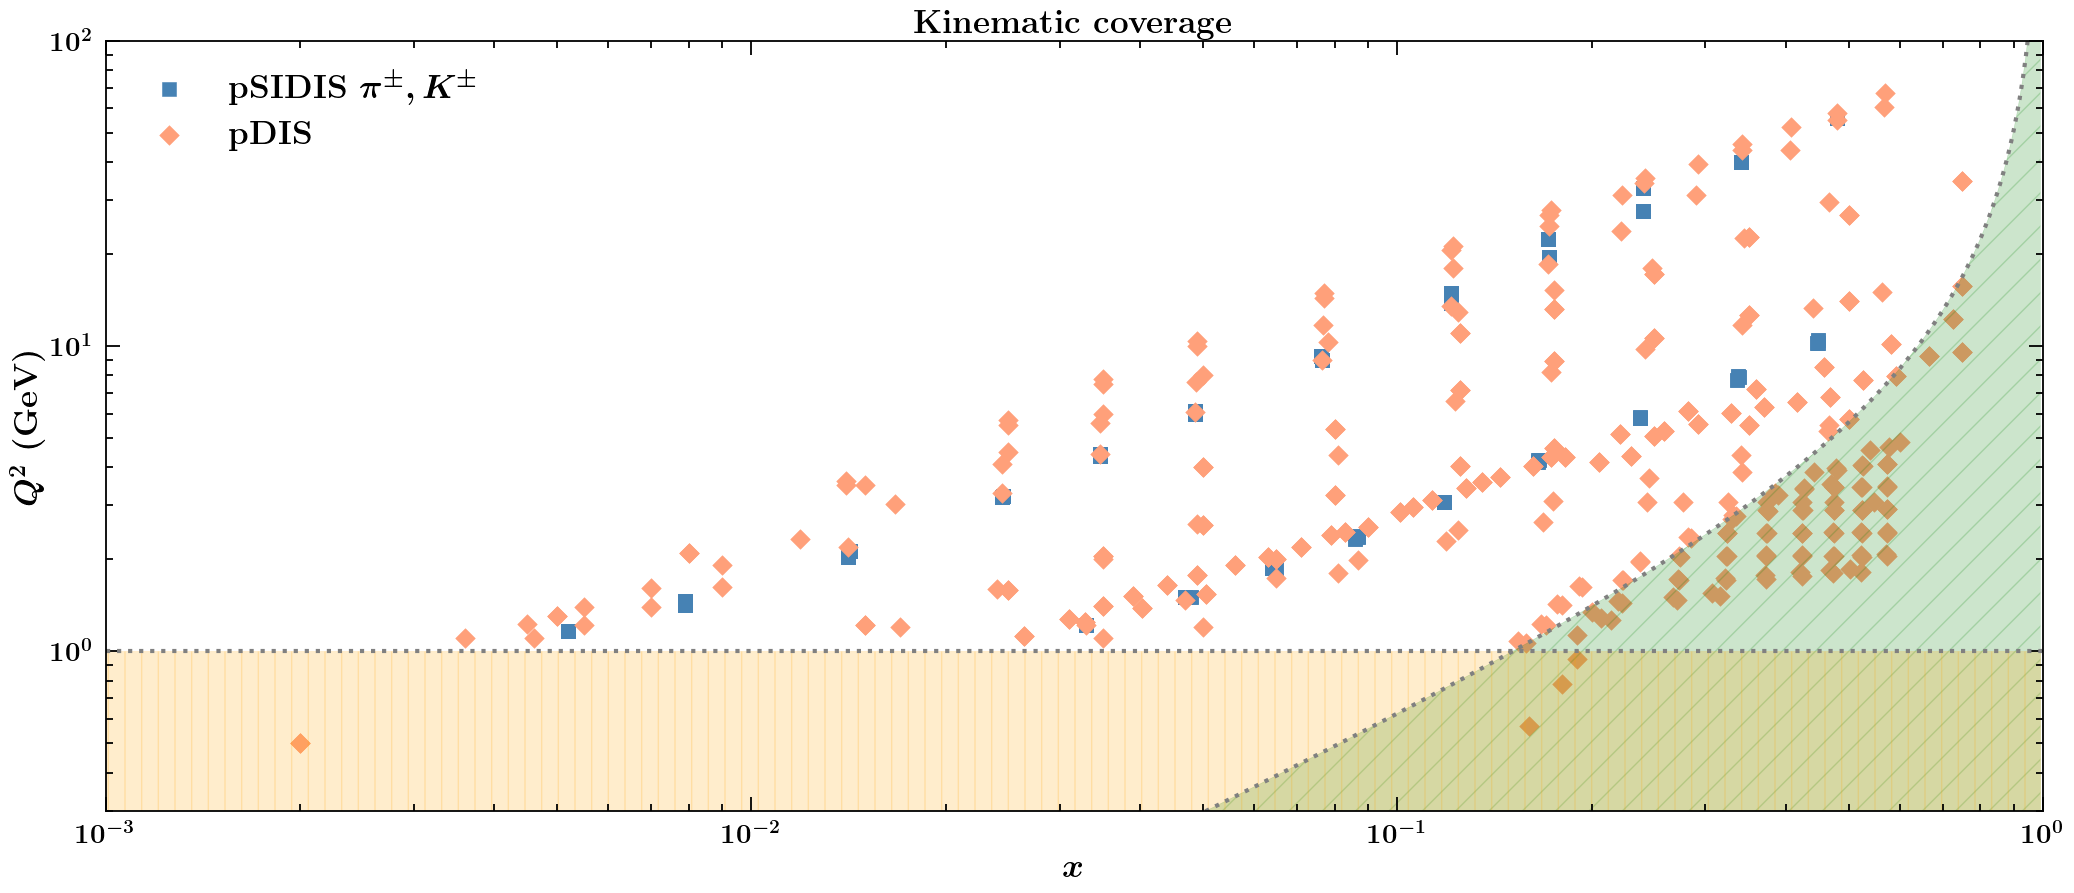
\includegraphics[width=1\textwidth]{kin_cov.png} 
  \caption{\small{Kinematic coverage in the $(x,Q^2)$ plane. The orange- and green-coloured areas represent the cuts in $Q^2$ and $W^2$, respectively.}}
  \label{fig:kin_cov}
\end{figure}
%%
The analysis makes use of inclusive and semi-inclusive lepton-nucleon DIS data coming from different facilities such as CERN \cite{EuropeanMuon:1989yki, SpinMuon:1999udj, COMPASS:2006mhr, COMPASS:2010wkz, COMPASS:2010hwr}, SLAC \cite{E142:1996thl, E143:1998hbs, E154:1997xfa, E155:2000qdr}, DESY \cite{HERMES:2018awh, HERMES:2006jyl, HERMES:1997hjr} and Jefferson Lab \cite{Kramer:2002tt, JeffersonLabHallA:2004tea, CLAS:2014qtg}. For both DIS and SIDIS, the lepton beams are made of either electrons or muons. The targets are either protons or neutrons, and, in some case, deuterons. The main features of the data sets are summarised in Tabs.~[\ref{tab:DIS_data}, \ref{tab:SIDIS_data}], in which the number of data points, the kinematic coverage, and the measured observables are shown. The global kinematic coverage in the $(x,Q^2)$ plane is also displayed in Fig.~\ref{fig:kin_cov}. \par
The observable adopted in the present work is the (semi-)inclusive structure function $g_1^{(h)}$. However, some experiments provide its value normalised to the unpolarised structure function, that is $g_1^{(h)}/F_1^{(h)}$. In this case, the predictions require the computation of the unpolarised structure function $F_1^{(h)}$ for each data point, which then divides the prediction for $g_1^{(h)}$. This introduces a dependence on the chosen unpolarised parton set.%

In order to ensure the reliability of perturbative QCD, all data points with $Q^2 \leq Q^2_{\T{cut}} = 1 \, \T{GeV}^2$ are excluded. This cut corresponds to the orange-coloured area of Fig.~\ref{fig:kin_cov}. In addition, I also impose a cut on the squared invariant mass of the hadronic final state $W^2$, in order to remove all the points that may be affected by higher-twist corrections, as discussed in \secref{sec:field_theoretic}. In choosing the value for $W_{\T{cut}}$, I performed several fits with different thresholds, that is $W_{\T{cut}}~=~1.0, \, 2.0, \, 2.5,$ and $3 \, \T{GeV}$. Although a small improvement of the fit quality (\textit{i.e.}, the global $\chi^2$ as I will discuss later) is observed as the cut on $W$ is raised, the impact on helicity PDFs remains however moderate. Thus, I chose to exclude points with $W^2~\leq~W^2_{\T{cut}}~=~6.5~\T{GeV}^2$ (green area in Fig.~\ref{fig:kin_cov}), which is a good compromise between the number of surviving points and the fit quality.%

The resulting kinematic coverage is highly affected by the cuts. Starting from $480$ initially available points, after cuts this number reduces to $N_{\T{dat}}=360$,  -- a reduction of about $25\%$ respect to the initial availability. It can be observed that the most affected experiments are those performed by Jefferson Lab \cite{Kramer:2002tt, JeffersonLabHallA:2004tea, CLAS:2014qtg}. Indeed, the cut in $W^2$ mainly affects all data points that cover the large-$x$ and small-$Q^2$ corner, which is exactly the region probed by these experiments.%

Although the coverage of both low- and large-$x$ regions have been improved in recent years, the present situation for polarised data is not comparable with the unpolarised counterpart. The latter provides over than $3000$ data points coming from different processes in addition to DIS (see \textit{e.g}, Ref.~\cite{Kassabov:2022pps}). Moreover, the accuracy of unpolarised measurements is generally better if compared to the polarised case. Still, this does not prevent us to perform a global determination, provided a reliable estimation of the uncertainties.%

For each observable listed in Tabs.~[\ref{tab:DIS_data},\ref{tab:SIDIS_data}], the experiments furnish information about their uncertainties. In particular, correlated systematics (multiplicative and/or additive) are only given by E143, E155, EMC, and HERMES, whereas the other experiments provide uncorrelated uncertainties only. The experimental covariance matrix $V_{ij}$ is constructed as follows
%%
\begin{equation}
  V_{ij} =  \sigma_{i,\T{unc}} \sigma_{j,\T{unc}} \delta_{ij} + \sum_{\ell=1}^{l} \sigma_{i,\T{corr}}^{(l)} \sigma_{j,\T{corr}}^{(\ell)} \,,
  \label{eq:covariance_matrix}
\end{equation}
%%
where $i$ and $j$ run over the experimental data points, $\sigma_{i,\T{corr}}^{(\ell)}$ are the various sources of correlated uncertainties, and $\sigma_{i,\T{unc}}$ are the uncorrelated uncertainties. The latter are defined as the sum in quadrature of all uncorrelated sources of statistical $\sigma_{i,\T{stat}}$ and systematic $\sigma_{i,\T{syst}}$ error for the $i$-th point
%%
\afterpage{
\begin{landscape}% Landscape page
  \begin{table}
  \scriptsize
  \centering % Center table
  \begin{tabularx}{1\pdfpagewidth}{llXXXcccc}
  \toprule \toprule
   Experiment    & Set  &  $N_{\T{dat}}$  &  $x_{\T{min}}$  &  $x_{\T{max}}$  & $Q^2_{\T{min}} [\T{GeV}^2]$ &  $Q^2_{\T{max}} [\T{GeV}^2]$ &    $F$    &  Ref. \\
  \midrule
   E142 
        \\       & E142-G1N & $8\,(7)$ & $.035$ & $.466$ & $1.1$ & $5.5$ & $g_1$ & \cite{E142:1996thl} \\
  \midrule
   E143 
        \\       &  E143-G1D  &   $28\,(25)$  &    $.031$       &      $.749$     &    $1.27$                   &       $9.52$                 &  $g_1$    & \cite{E143:1998hbs} \\       
                 &  E142-G1P  &   $28\,(25)$  &    $.035$       &      $.466$     &    $1.27$                   &       $9.52$                 &  $g_1$    & \cite{E143:1998hbs} \\
  \midrule
   E154 
        \\       &  E154-G1N  &   $11$         &    $.017$      &      $.024$      &   $ 1.2$                    & $15.0$                       & $g_1$     & \cite{E154:1997xfa} \\
  \midrule
   E155 
       \\        & E155-A1P   & $24\,(22)$      & $.015$        & $.750$          &  $1.22$                & $34.72$                & $g_1/F_1$          & \cite{E155:2000qdr}
       \\        & E155-A1N   & $24\,(22)$      & $.015$        & $.750$          &  $1.22$                & $34.72$                & $g_1/F_1$          & \cite{E155:2000qdr} \\
  \midrule
   EMC 
       \\        & EMC-G1P    & $10$         & $.015$       & $0.466$       &    $3.5$         & $29.5$                      & $g_1$          & \cite{EuropeanMuon:1989yki} \\
  \midrule
   JLAB E06 014
       \\        & JLAB-A1N   & $6\,(1)$     & $.277$       & $0.548$      & $3.078$    & $3.078$                  & $g_1/F_1$  & \cite{JeffersonLabHallA:2016neg} \\
  \midrule
   JLAB E97 103
       \\        & JLAB-E97-103-G1N & $5\,(0)$ & $.160$ & $.200$ & $0.57$ & $1.34$ & $g_1$ & \cite{Kramer:2002tt}\\
  \midrule
   JLAB E99 117 
       \\        & JLAB-E99-117-G1N-F1N & $3\,(0)$ & $.33$ & $.60$ & $2.71$ & $4.83$ & $g_1/F_1$ & \cite{JeffersonLabHallA:2004tea} \\
  \midrule
   JLAB EG1 DVCS-D 
       \\        & JLAB-EG1-DVCS-G1D-F1D & $44\,(1)$ & $.158$ & $0.574$ & $1.078$ & $4.666$ & $g_1/F_1$ & \cite{CLAS:2014qtg}
       \\        & JLAB-EG1-DVCS-G1P-F1P & $47\,(2)$ & $.154$ & $0.578$ & $1.064$ & $4.115$ & $g_1/F_1$ & \cite{CLAS:2014qtg} \\
  \midrule
   SMC
       \\        & SMC-G1D & $13\,(12)$ & $.002$ & $.48$ & $0.50$ & $54.80$ & $g_1$ &  \cite{SpinMuon:1999udj} 
       \\        & SMC-G1P & $13\,(12)$ & $.002$ & $.48$ & $0.50$ & $54.80$ & $g_1$ &  \cite{SpinMuon:1999udj} \\
  \midrule 
   COMPASS-D
       \\        & CMP07-G1D & $15$ & $.0046$ & $0.567$ & $1.1$ & $60.8$ & $g_1$ & \cite{COMPASS:2006mhr} \\
  \midrule
   COMPASS-P 
       \\        & CMP10-G1P & $17$ & $.0036$ & $.57$ & $1.1$ & $67.4$ & $g_1$ & \cite{COMPASS:2010wkz} \\
  \midrule 
   HERMES97 
       \\        & HERMES-G1N & $9\,(8)$ & $.033$ & $.464$ & $1.22$ & $5.25$ & $g_1$ & \cite{HERMES:1997hjr} \\
  \midrule
   HERMES 
       \\        & HERMES-G1P & $15\,(14)$ & $.0264$ & $.7248$ & $1.12$ & $12.21$ & $g_1$ & \cite{HERMES:2006jyl} 
       \\        & HERMES-G1D & $15\,(14)$ & $.0264$ & $.7248$ & $1.12$ & $12.21$ & $g_1$ & \cite{HERMES:2006jyl} \\
  \midrule
   Total DIS         &    & $335 \, (218)$  & & &  &    &      &      \\
  \bottomrule
\end{tabularx}
  \caption{
    \small
    Experimental DIS data sets included in the \texttt{MAPpol1.0} analysis. For each experiment, the number of data points before and after (in parentheses) applying kinematic cuts, the covered kinematic range and the measured observables are shown.
  \label{tab:DIS_data}}% Add 'table' caption
  \end{table}
\end{landscape}}
%%
\afterpage{
\begin{landscape}% Landscape page
  \begin{table}
  \scriptsize
  \centering % Center table
  \begin{tabularx}{1\pdfpagewidth}{llXXXcccc}
  \toprule \toprule
   Experiment    & Set       &  $N_{\T{dat}}$  &  $x_{\T{min}}$  &  $x_{\T{max}}$  & $Q^2_{\T{min}} [\T{GeV}^2]$ &  $Q^2_{\T{max}} [\T{GeV}^2]$ &    $F$    &  Ref. \\
  \midrule
   COMPASS-P 
     \\          & COMPASS-A1P-KA-MINUS & $12$ & $.004$ & $.7$ & $1.16$ & $55.6$ & $g_1^{(h)}/F_1^{(h)}$ & \cite{COMPASS:2010hwr} \\
                 & COMPASS-A1P-KA-PLUS & $12$ & $.004$ & $.7$ & $1.16$ & $55.6$ & $g_1^{(h)}/F_1^{(h)}$ & \cite{COMPASS:2010hwr} \\
                 & COMPASS-A1P-PI-MINUS & $12$ & $.004$ & $.7$ & $1.16$ & $55.6$ & $g_1^{(h)}/F_1^{(h)}$ & \cite{COMPASS:2010hwr} \\
                 & COMPASS-A1P-PI-PLUS & $12$ & $.004$ & $.7$ & $1.16$ & $55.6$ & $g_1^{(h)}/F_1^{(h)}$ & \cite{COMPASS:2010hwr} \\
  \midrule
   COMPASS-D 
     \\          & COMPASS-A1D-KA-MINUS & $10$ & $.004$ & $.7$ & $1.16$ & $32.8$ & $g_1^{(h)}/F_1^{(h)}$ & \cite{COMPASS:2010hwr} \\
                 & COMPASS-A1D-KA-PLUS & $10$ & $.004$ & $.7$ & $1.16$ & $32.8$ & $g_1^{(h)}/F_1^{(h)}$ & \cite{COMPASS:2010hwr} \\
                 & COMPASS-A1D-PI-MINUS & $10$ & $.004$ & $.7$ & $1.16$ & $32.8$ & $g_1^{(h)}/F_1^{(h)}$ & \cite{COMPASS:2010hwr} \\
                 & COMPASS-A1D-PI-PLUS & $10$ & $.004$ & $.7$ & $1.16$ & $32.8$ & $g_1^{(h)}/F_1^{(h)}$ & \cite{COMPASS:2010hwr} \\
  \midrule
   HERMES-P 
     \\          & HERMES-2018-A1P-PI-MINUS & $9$ & $.033$ & $.449$ & $1.22$ & $10.28$ & $g_1^{(h)}/F_1^{(h)}$ & \cite{HERMES:2018awh} \\
                 & HERMES-2018-A1P-PI-PLUS & $9$ & $.033$ & $.449$ & $1.22$ & $10.17$ & $g_1^{(h)}/F_1^{(h)}$ & \cite{HERMES:2018awh} \\ 
  \midrule
   HERMES-D 
     \\          & HERMES-2018-A1D-KA-MINUS & $9$ & $.033$ & $.449$ & $1.21$ & $10.01$ & $g_1^{(h)}/F_1^{(h)}$ & \cite{HERMES:2018awh} \\
                 & HERMES-2018-A1D-KA-PLUS & $9$ & $.033$ & $.449$ & $1.21$ & $10.07$ & $g_1^{(h)}/F_1^{(h)}$ & \cite{HERMES:2018awh} \\
                 & HERMES-2018-A1D-PI-MINUS & $9$ & $.033$ & $.449$ & $1.21$ & $9.97$ & $g_1^{(h)}/F_1^{(h)}$ & \cite{HERMES:2018awh} \\
                 & HERMES-2018-A1D-PI-PLUS & $9$ & $.033$ & $.449$ & $1.21$ & $9.92$ & $g_1^{(h)}/F_1^{(h)}$ & \cite{HERMES:2018awh}\\
  \midrule
   Total  SIDIS        &    & $142$  &      &      &         &     &     &      \\
  \midrule \toprule
   \\[0.5pt]
   Total & & $477 \, (360)$ & & & & & & \\
  \bottomrule
\end{tabularx}
  \caption{
    \small
    Experimental SIDIS data sets included in the \texttt{MAPpol1.0} analysis. For each experiment, show the number of data points before and after (in parenthesis) applying kinematic cuts, the covered kinematic range and the measured observables are shown.
  \label{tab:SIDIS_data}}% Add 'table' caption
  \end{table}
\end{landscape}}
%%
\begin{equation}
  \sigma_{i,\T{unc}}^2 = \sigma_{i,\T{stat}}^2 + \sigma_{i,\T{syst}}^2 \,.
\end{equation}
%%
Finally, I anticipate that the first moments of the non-singlet triplet and octet distributions, $a_3$ and $a_8$, are treated as two additional data points that enter the computation of the $\chi^2$. The values, measured from the hyperon $\beta$-decay, are \cite{Nakamura_2010}
%%
\begin{equation}
  a_3 = 1.2701 \pm 0.0025 \hspace{10mm} a_8 = 0.585 \pm 0.025 \,.
  \label{eq:a3_a8_values}
\end{equation}
%%
I will further discuss these two points in \secref{sec:4.3}.

\subsection*{Generation of Monte Carlo replicas}
In order to propagate the error from experimental data, we use the Monte Carlo sampling method discussed in \secref{sec:MAP}. The artificial points are obtained by sampling the distributions of experimental data, obtaining an ensemble of $N_{\T{rep}}$ replicas that reflects the statistical properties of the original data set.%

The key point to observe is that the fluctuated points must follow the same distribution of the unfluctuated data. I assume data to be distributed according to a multi-variate Gaussian distribution, whose mean values correspond to the experimental central points and the covariance matrix is constructed as in Eq.~\eqref{eq:covariance_matrix}. The $\chi^2$ obtained by comparing the unfluctuated central value $m_j$ with its fluctuated value $f_j$, expressed in matrix form, must then read
%%
\begin{equation}
  \chi^2 = \tran{\vb*{d}} \cdot \vb*{V}^{-1} \cdot \vb*{d} \,,
  \label{eq:chi_fluc}
\end{equation}
%%
where $\vb*{V}$ is the usual $N_{\T{dat}} \times N_{\T{dat}}$ covariance matrix and $\vb*{d}$ is a column vector with $N_{\T{dat}}$ entries defined as
%%
\begin{equation}
  d_j = f_j - m_j \,.
\end{equation}
%%
On the other hand, the $\chi^2$ is also defined as
%%
\begin{equation}
  \chi^2 = \sum_{i=1}^{N_{\T{dat}}} z_i^2 = \left| \vb*{z} \right|^2 \,,
  \label{eq:chi2_normal}
\end{equation}
%%
where $z_j$ are independent, standard normal random variables such that
%%
\begin{equation}
  \langle z_i \rangle = 0 \hspace{10mm} \T{and} \hspace{10mm}  \langle z_i z_j \rangle = \delta_{ij} \,.
\end{equation}
%%
It immediately follows that $\langle \chi^2 \rangle = N_{\T{dat}}$, as predicted by the $\chi^2$ distribution. Now, the covariance matrix, being a symmetric object, admits the so called Cholesky decomposition, that allows us to write
%%
\begin{equation}
  \vb*{V} = \vb*{L} \cdot \tran{\vb*{L}} \,,
\end{equation}
%%
where $\vb*{L}$ is a lower diagonal matrix\footnote{Further details on the Cholesky decomposition can be found in Appendix \ref{app:lin_sys}.}. Thus, the $\chi^2$ in Eq.~\eqref{eq:chi_fluc} can be recast as
%%
\begin{equation}
  \chi^2 = \left| \vb*{L}^{-1} \cdot \vb*{d} \right|^2 \,.
  \label{eq:chi2_Cholesky}
\end{equation}
%%
Collecting Eqs.~\eqref{eq:chi2_Cholesky} and \eqref{eq:chi2_normal}, one finally obtains the following relation
%%
\begin{equation}
  f_j = m_j + \sum_{i=1}^{N_{\T{dat}}} L_{ji} z_i\,.
  \label{eq:MC_gen}
\end{equation}
%%
We stress that the above expression has been obtained by imposing that the fluctuated data followed the multi-variate Gaussian distribution and that the $\chi^2$ had the correct distribution. Thus, in order to generate an artificial value $f_j$, one has to use Eq.~\eqref{eq:MC_gen}, where $z_j$ is randomly extracted from a centred, univariate Gaussian distribution.\par
It is straightforward to show that the fluctuations generated according to Eq.~\eqref{eq:MC_gen} present the same statistical properties of the original data set. In particular, one can show that
%%
\begin{gather}
  \langle f_j \rangle = m_j \,,\\
  \langle f_j f_k \rangle = \langle f_j \rangle \langle f_k \rangle + V_{jk} \,,
\end{gather}
%%
which are the expected relations for a correct generation of a Monte Carlo ensemble.

%
\afterpage{
  \begin{figure}[t]
    \centering
    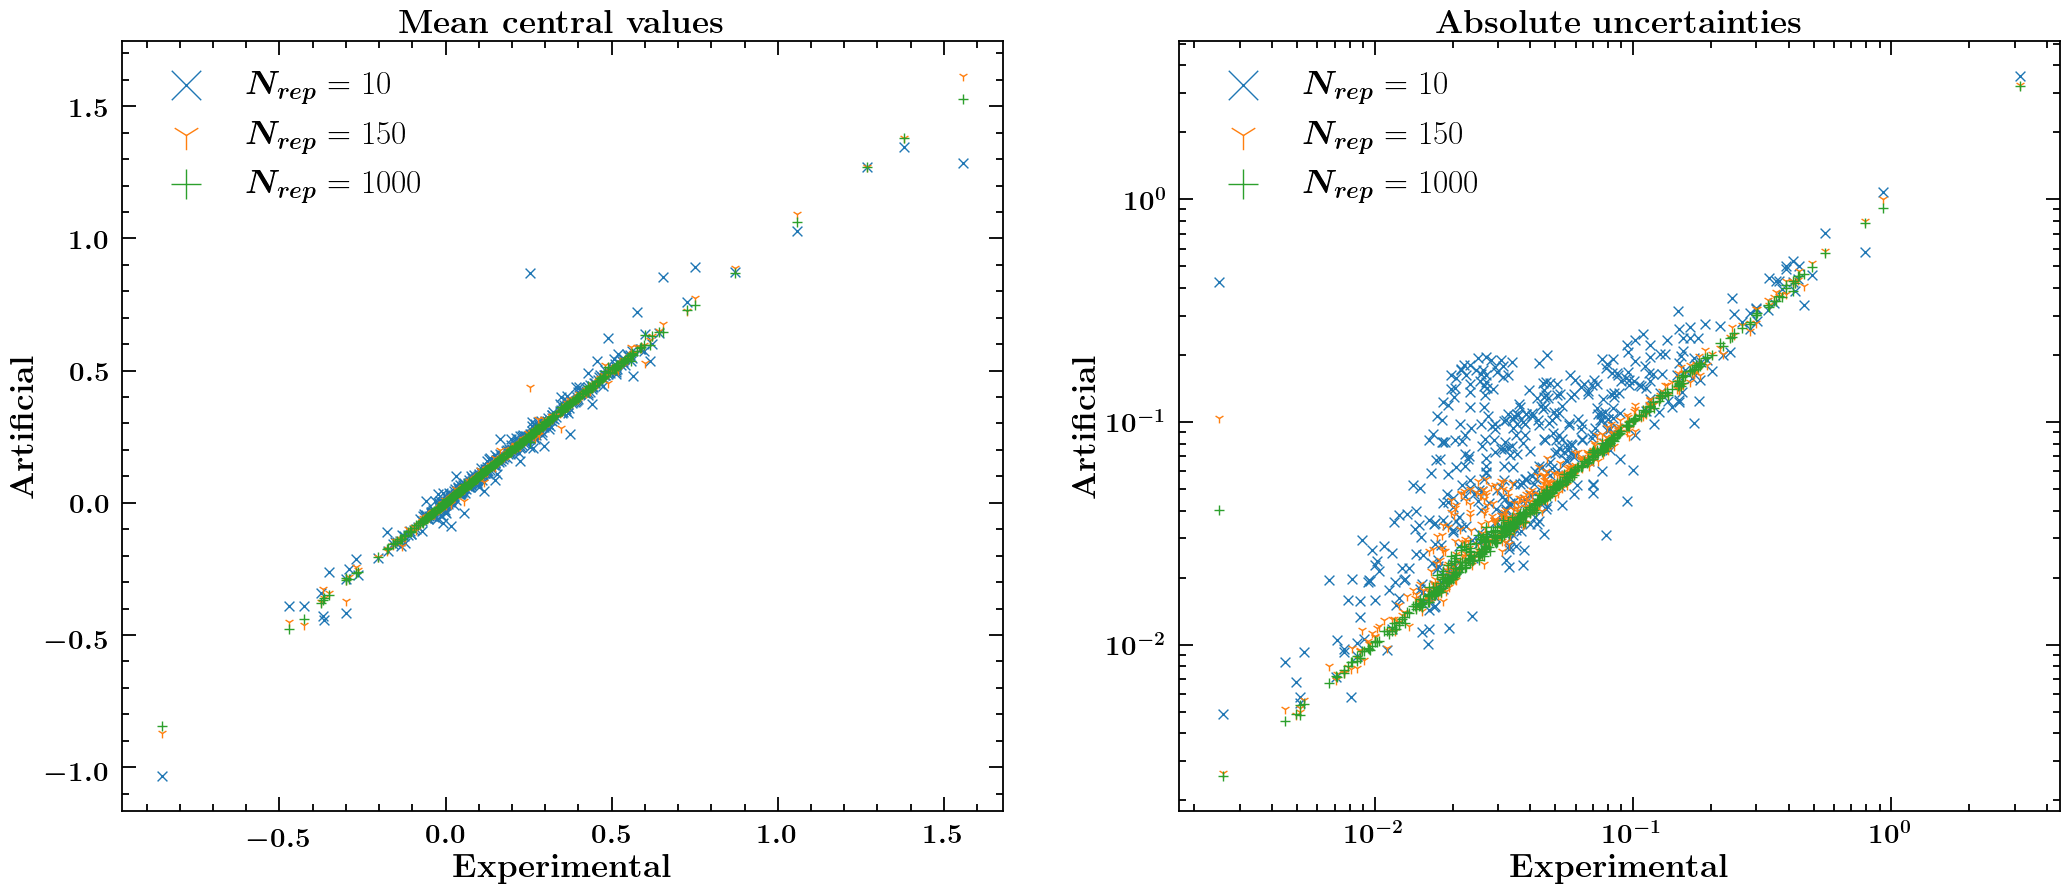
\includegraphics[width=1\textwidth]{replica_number.png} 
    \caption{\small{Scatter plots of experimental versus artificial Monte Carlo mean central values and absolute uncertainties of polarized structure functions computed from ensembles made of $N_{\T{rep}} = 10$, $100$, $1000$ replicas.\\}
    \vspace{1cm}}
    \label{fig:replica_number}
  \end{figure}
  %%
  \begin{table}[b]
    \scriptsize
    \centering % Center table
    \begin{tabular}{lccc@{\hspace{1cm}}ccc}
  \toprule \toprule
   Experiment    & \multicolumn{3}{c}{$\left< \T{PE} \left[ \left<F^{\T{(art)}} \right>  \right] \right> [\%]$} & \multicolumn{3}{c}{$r \left[ F^{\T{(art)}} \right]$}\\[10pt]
  \toprule
                      &    10     &     150   &    1000  &    10     &     150   &    1000  \\
  \midrule
      COMPASS-P $K^-$   &   24.1    &     4.6   &    4.2   &  .96321  &  .99928  &  .99986 \\
      COMPASS-P $K^+$   &    3.8    &     0.9   &    0.8   &  .99829  &  .99996  &  .99992 \\
    COMPASS-P $\pi^-$   &    5.0    &     1.0   &    0.4   &  .99824  &  .99945  &  .99997 \\
    COMPASS-P $\pi^+$   &    4.9    &     0.7   &    0.1   &  .99916  &  .99993  &  .99999 \\
      COMPASS-D $K^-$   &   41.3    &    14.5   &    3.6   &  .81885  &  .99071  &  .99740 \\
      COMPASS-D $K^+$   &    4.4    &     0.8   &    0.3   &  .98961  &  .99958  &  .99990 \\
    COMPASS-D $\pi^-$   &    9.1    &     1.2   &    0.5   &  .99187  &  .99955  &  .99999 \\
    COMPASS-D $\pi^+$   &    3.8    &     0.8   &    0.5   &  .99538  &  .99991  &  .99997 \\
      HERMES-D  $K^-$   &   10.4    &     1.4   &    0.6   &  .99724  &  .99994  &  .99996 \\
      HERMES-D  $K^+$   &    1.9    &     0.5   &    0.2   &  .99841  &  .99995  &  .99998 \\
    HERMES-D  $\pi^-$   &    2.8    &     0.9   &    0.2   &  .98590  &  .99877  &  .99998 \\
    HERMES-D  $\pi^+$   &    3.1    &     0.6   &    0.2   &  .99641  &  .99980  &  .99998 \\
    HERMES-P  $\pi^-$   &    1.0    &     0.2   &    0.1   &  .99608  &  .99657  &  .99986 \\
    HERMES-P  $\pi^+$   &    0.5    &     0.1   &    0.0   &  .99389  &  .99996  &  .99999 \\
               E143-D   &    2.6    &     0.8   &    0.3   &  .98091  &  .99891  &  .99988 \\
               E143-P   &    0.4    &     0.2   &    0.0   &  .99927  &  .99978  &  .99999 \\
               E154-N   &    0.9    &     0.2   &    0.1   &  .99346  &  .99987  &  .99996 \\
               E155-P   &    0.4    &     0.1   &    0.1   &  .99912  &  .99984  &  .99987 \\
               E155-N   &   10.8    &     1.7   &    0.8   &  .91095  &  .98952  &  .99951 \\
                EMC-P   &    0.6    &     0.3   &    0.0   &  .99228  &  .99775  &  .99994 \\
         JLAB E06 014   &    4.7    &     0.4   &    0.1   &  .97261  &  .99955  &  .99997 \\
         JLAB E97 103   &    0.1    &     0.0   &    0.0   &  .99944  &  .99968  &  .00000 \\
         JLAB E99 117   &    0.2    &     0.0   &    0.0   &  .99605  &  .99979  &  .99993 \\
      JLAB EG1 DVCS-D   &    0.6    &     0.2   &    0.1   &  .99855  &  .99990  &  .99999 \\
      JLAB EG1 DVCS-P   &    0.2    &     0.1   &    0.0   &  .99979  &  .99998  &  .00000 \\
                SMC-D   &    0.8    &     0.2   &    0.1   &  .97954  &  .99434  &  .99973 \\
                SMC-P   &    0.2    &     0.1   &    0.0   &  .99522  &  .99918  &  .99980 \\
            COMPASS-P   &    0.2    &     0.1   &    0.0   &  .99747  &  .99899  &  .99976 \\
             HERMES-N   &    0.8    &     0.1   &    0.1   &  .99377  &  .99971  &  .99987 \\
             HERMES-D   &    0.5    &     0.1   &    0.0   &  .99562  &  .99929  &  .99991 \\
             HERMES-P   &    0.1    &     0.0   &    0.0   &  .99854  &  .99985  &  .99999 \\
  \midrule \bottomrule
\end{tabular}
    \caption{
      \small
      Table of statistical estimators for the mean value computed from the Monte Carlo sample with $N_{\T{rep}}=10,\, 150,\, 1000$ replicas.
    \label{tab:PE}}% Add 'table' caption
  \end{table}
  \clearpage
}
%
The number of replicas is chosen in order to faithfully reproduce the statistical estimators of the original experimental data. For instance, one can check if the averages and the variances of the replica sample, that is
%%
\begin{equation}
  \langle F_{i}^{\T{(art)}} \rangle = \frac{1}{N_{\T{rep}}} \sum_{k=1}^{N_{\T{rep}}} F_{i}^{(k)} \hspace{5mm} \T{and} \hspace*{5mm} \sigma_i^{\T{(art)}} = \sqrt{ \langle \left( F_{i}^{\T{(art)}} \right) \rangle - \langle F_{i}^{\T{(art)}} \rangle^2} \,,
\end{equation}
%%
reproduce the experimental central values and the uncertainties of the original data set. Such a comparison is shown in Fig.~\ref{fig:replica_number}, where I display scatter plots of the central values and errors for sample of $N_{\T{rep}} = 10$, $150$ and $1000$ replicas. Although they only provide a qualitative description, they clearly show that the accuracy of the artificial sample increases with the size of the Monte Carlo sample. A more quantitative description can be carried out by defining appropriate statistical estimators. Following Ref.~\cite{DelDebbio:2004xtd}, I make use of the percentage error and the scatter correlation r for central values, whose definitions are
%
\begin{gather}
  \left< PE \left[ \left< F^{(\T{art})} \right>_{\T{rep}} \right] \right>_{\T{dat}} = \frac{1}{N_{\T{dat}}} \sum_{i=1}^{N_{\T{dat}}} \frac{\abs{\left< F_i^{\T{(art)}} \right>_{\T{rep}} - F_{i}^{\T{(exp)}}}}{F_i^{\T{(exp)}}}\,, \\
  r \left[ F^{\T{(art)}} \right] = \frac{\left< F^{\T{(exp)}} \left< F^{\T{(art)}} \right>_{\T{rep}} \right>_{\T{dat}} - \left< F^{\T{(exp)}} \right>_{\T{dat}} \left<  \left< F^{\T{(art)}} \right>_{\T{(rep)}}\right>_{\T{dat}} }{\sigma_s^{\T{(exp)}} \sigma_s^{\T{(art)}} }\,,
\end{gather}
%%
where the scatter variances are defined as
%%
\begin{gather}
  \sigma^{\T{(exp)}}_s = \sqrt{\left< \left( F^{\T{(exp)}} \right)^2 \right>_{\T{dat}} - \left( \left< F^{\T{(exp)}} \right>_{\T{dat}} \right)^2} \,,\\
  %
  \sigma^{\T{art}}_s = \sqrt{\left< \left( \left<F^{\T{(art)}}\right>_{\T{rep}} \right)^2 \right>_{\T{dat}} - \left( \left< \left<F^{\T{(art)}}\right>_{\T{rep}} \right>_{\T{(dat)}} \right)^2} \,.
\end{gather}
%%
Essentially, the percentage error describes how well the central values are recovered by the Monte Carlo sample. On the other hand, the scatter correlation $r$ reflects the capacity of the Monte Carlo sample to reproduce the correlations that are present in the original data set. For each experiment, I show these two values for the observables $g_1^{(h)}$ and $g_1^{(h)}/F_1^{(h)}$ in Tab.~\ref{tab:PE}. The Monte Carlo sample with size $N_{\T{rep}} = 150$ gives a satisfactory reproduction of mean values and uncertainties of experimental data. The improvements obtained by using a larger sample are moderate, and, in any case, do not justify the higher computational effort. For these reasons, I will henceforth adopt the ensemble with $N_{\T{rep}} = 150$ replicas as the standard configuration for the presented fits.

%_________________________________
\section{Details of the QCD analysis}
\label{sec:4.2}
Here I summarise the aspects concerning the QCD analysis of polarised structure functions. The main observables used throughout the analysis are the structure functions $g_1$, Eq.~\eqref{eq:g1_QFT}, and $g_1^h$, Eq.~\eqref{eq:g1h}, for DIS and SIDIS respectively. They are expressed in terms of combinations of PDFs and provide complementary constraints on the distributions.%

On the one hand, data coming from DIS experiments constraints only the linear combination of $\Delta \Sigma$, $\Delta T_3$, $\Delta T_8$, together with $\Delta g$, as it can be easily seen from Eq.~\eqref{eq:g1_NPM_ev}. On the other hand, SIDIS data provides full flavour separation. Moreover, given that data with kaons in the final state are given, the constraining power for the strange distributions $\Delta s$ and $\Delta \bar{s}$ is strengthened. In both SIDIS and DIS processes, the gluon distribution $\Delta g$ is weakly constrained. Indeed, it enters at NLO and its effect is lessened by the running coupling. Processes other than those we have just discussed (such as jet or semi-inclusive production in proton-proton collisions), receiving LO contributions from gluon initiated subprocesses, may provide direct information on the gluon distribution \cite{Rojo:2015acz}.%

Since we use data with different targets, we must take into account the hadron that PDFs refer to. The proton, neutron, and deuteron PDFs are related to each other by isoscalarity (assumed as an exact symmetry) so that
%%
\begin{equation}
  \begin{split}
    &\Delta u^{(I)} = I \Delta u^p + ( 1 - I ) \Delta d^p \\
    &\Delta d^{(I)} = I \Delta d^p + ( 1 - I ) \Delta u^p
  \end{split}
  \label{eq:iso_rel}
\end{equation}
%%
where $I=1$, $0.5$ and $0$ representing proton, deuteron, and neutron respectively. A similar relation also holds for antiquark distributions. We will henceforth assume that PDFs refer to the proton. The other distributions can be obtained by means of Eqs.~\eqref{eq:iso_rel}.%

Since both $\Delta s$ and $\Delta \bar{s}$ are sea-distributions for all targets, I assume that
%%
\begin{equation}
  \Delta s = \Delta \bar{s} \,,
\end{equation}
%%
which simplifies the analysis. The analysis has been carried out neglecting heavy quark distributions, which have been fixed to zero. The value for the strong coupling constant has been fixed to $\alpha_s(M_Z^2) = 0.118$.%

Finally, the computation of SIDIS observables requires the introduction of fragmentation functions sets. For this analysis, I make use of the pion and kaon fragmentation functions sets \texttt{MAPFF1.0} obtained from a global analysis performed at next-to-next-to-leading order accuracy~\cite{Khalek:2021gxf, AbdulKhalek:2022laj}.

\section{Fitting configuration}
\label{sec:4.3}
In this section, I give the details of the fitting configuration adopted in the \texttt{MAPPol1.0} analysis. I discuss which flavours are taken into account and how the distributions are parametrised in terms of a neural network. Then, I will move to the description of the training procedure, providing a more detailed picture than that given in \secref{sec:NNtr}. In particular, I will describe the difference between the error function, used during the minimisation, and the global $\chi^2$, used to assess the fit quality. Finally, I review the theoretical constraints assumed in the analysis and their implications.

\subsection*{Neural Network parametrisation}
The six independent distributions that are determined through the analysis are $\Delta u, \, \Delta d, \, \Delta s, \, \Delta \bar{u}, \, \Delta \bar{d}$ and $\Delta g$. These distributions are parametrised in terms of a single multi-layer feed-forward neural network, whose output layer is compounded of six differential nodes, one for each distribution. The PDFs are parametrised at an initial scale $\mu_0 = 1\,\T{GeV}$. The output of the network is then evolved to the experimental scale by means of the DGLAP equations, Eq.~\eqref{eq:DGLAP_coupled}. It has been observed that the variation of the initial scale up to $\mu_0 = 1.5\,\T{Gev}$ does not enhance the fit quality and the impact on PDFs is moderate. Higher values of the initial scale have not been considered, since heavy quark distributions would no longer be negligible\footnote{\footnotesize{The threshold over which heavy quark distributions start to contribute is fixed to the quark masses, $m_c=1.51\, \T{GeV}$ and $m_b=4.92\, \T{GeV}$.}}.%

The architecture of the neural network is 1-10-6, which introduces 86 free parameters. I explicitly verified the parametrisation to be redundant enough to ensure that the results do not depend on the architecture. Indeed, keeping on the single deep-layer structure, I have not observed any considerable difference in the results by either increasing the nodes of the internal layer up to 20 or reducing this number to 5. Thus, an architecture with 10 internal nodes is a good compromise between the number of parameters and the redundancy in the parametrisation, which is enough to reproduce any functional form given sufficient training time.%

The single node in the input layer corresponds to the Bjorken variable $x$\footnote{\footnotesize{Other determinations supplement the above parametrisation with a preprocessing function. This consists of multiplying the neural network by a fixed function that reflects some known behaviour of the distributions. For instance, the \texttt{NNPDFpol1.1} analysis from NNPDF collaboration \cite{Nocera:2014gqa} introduces these functions to enforce specific small- and large-x behaviours on parton distributions.}}. All the nodes except for the input one use a sigmoid as activation function, Eq.~\eqref{eq:sigmoid}. However, the output nodes of the last layer have been slightly modified in order to constraint to zero parton distributions at $x=1$ and to implement, analytically, the positivity constraint (see later).%

Finally, it is worth noting that there are as many networks as the number of replicas that have been generated. In this case, there are 150 neural networks, representing the statistical ensemble of polarised PDFs. Since dealing with such a huge number of networks is a heavy computational task, the outputs of the network (\textit{i.e.}, the PDFs) are put on a grid in the $(x,Q^2)$ plane. The value for an arbitrary pair $(x,Q^2)$ can be easily accessed through the LHAPDF interface \cite{Buckley:2014ana}. A schematic representation of the fitting algorithm is sketched in Fig.~\ref{fig:NN_plot}.
%%
\begin{figure}[t]
  \centering
  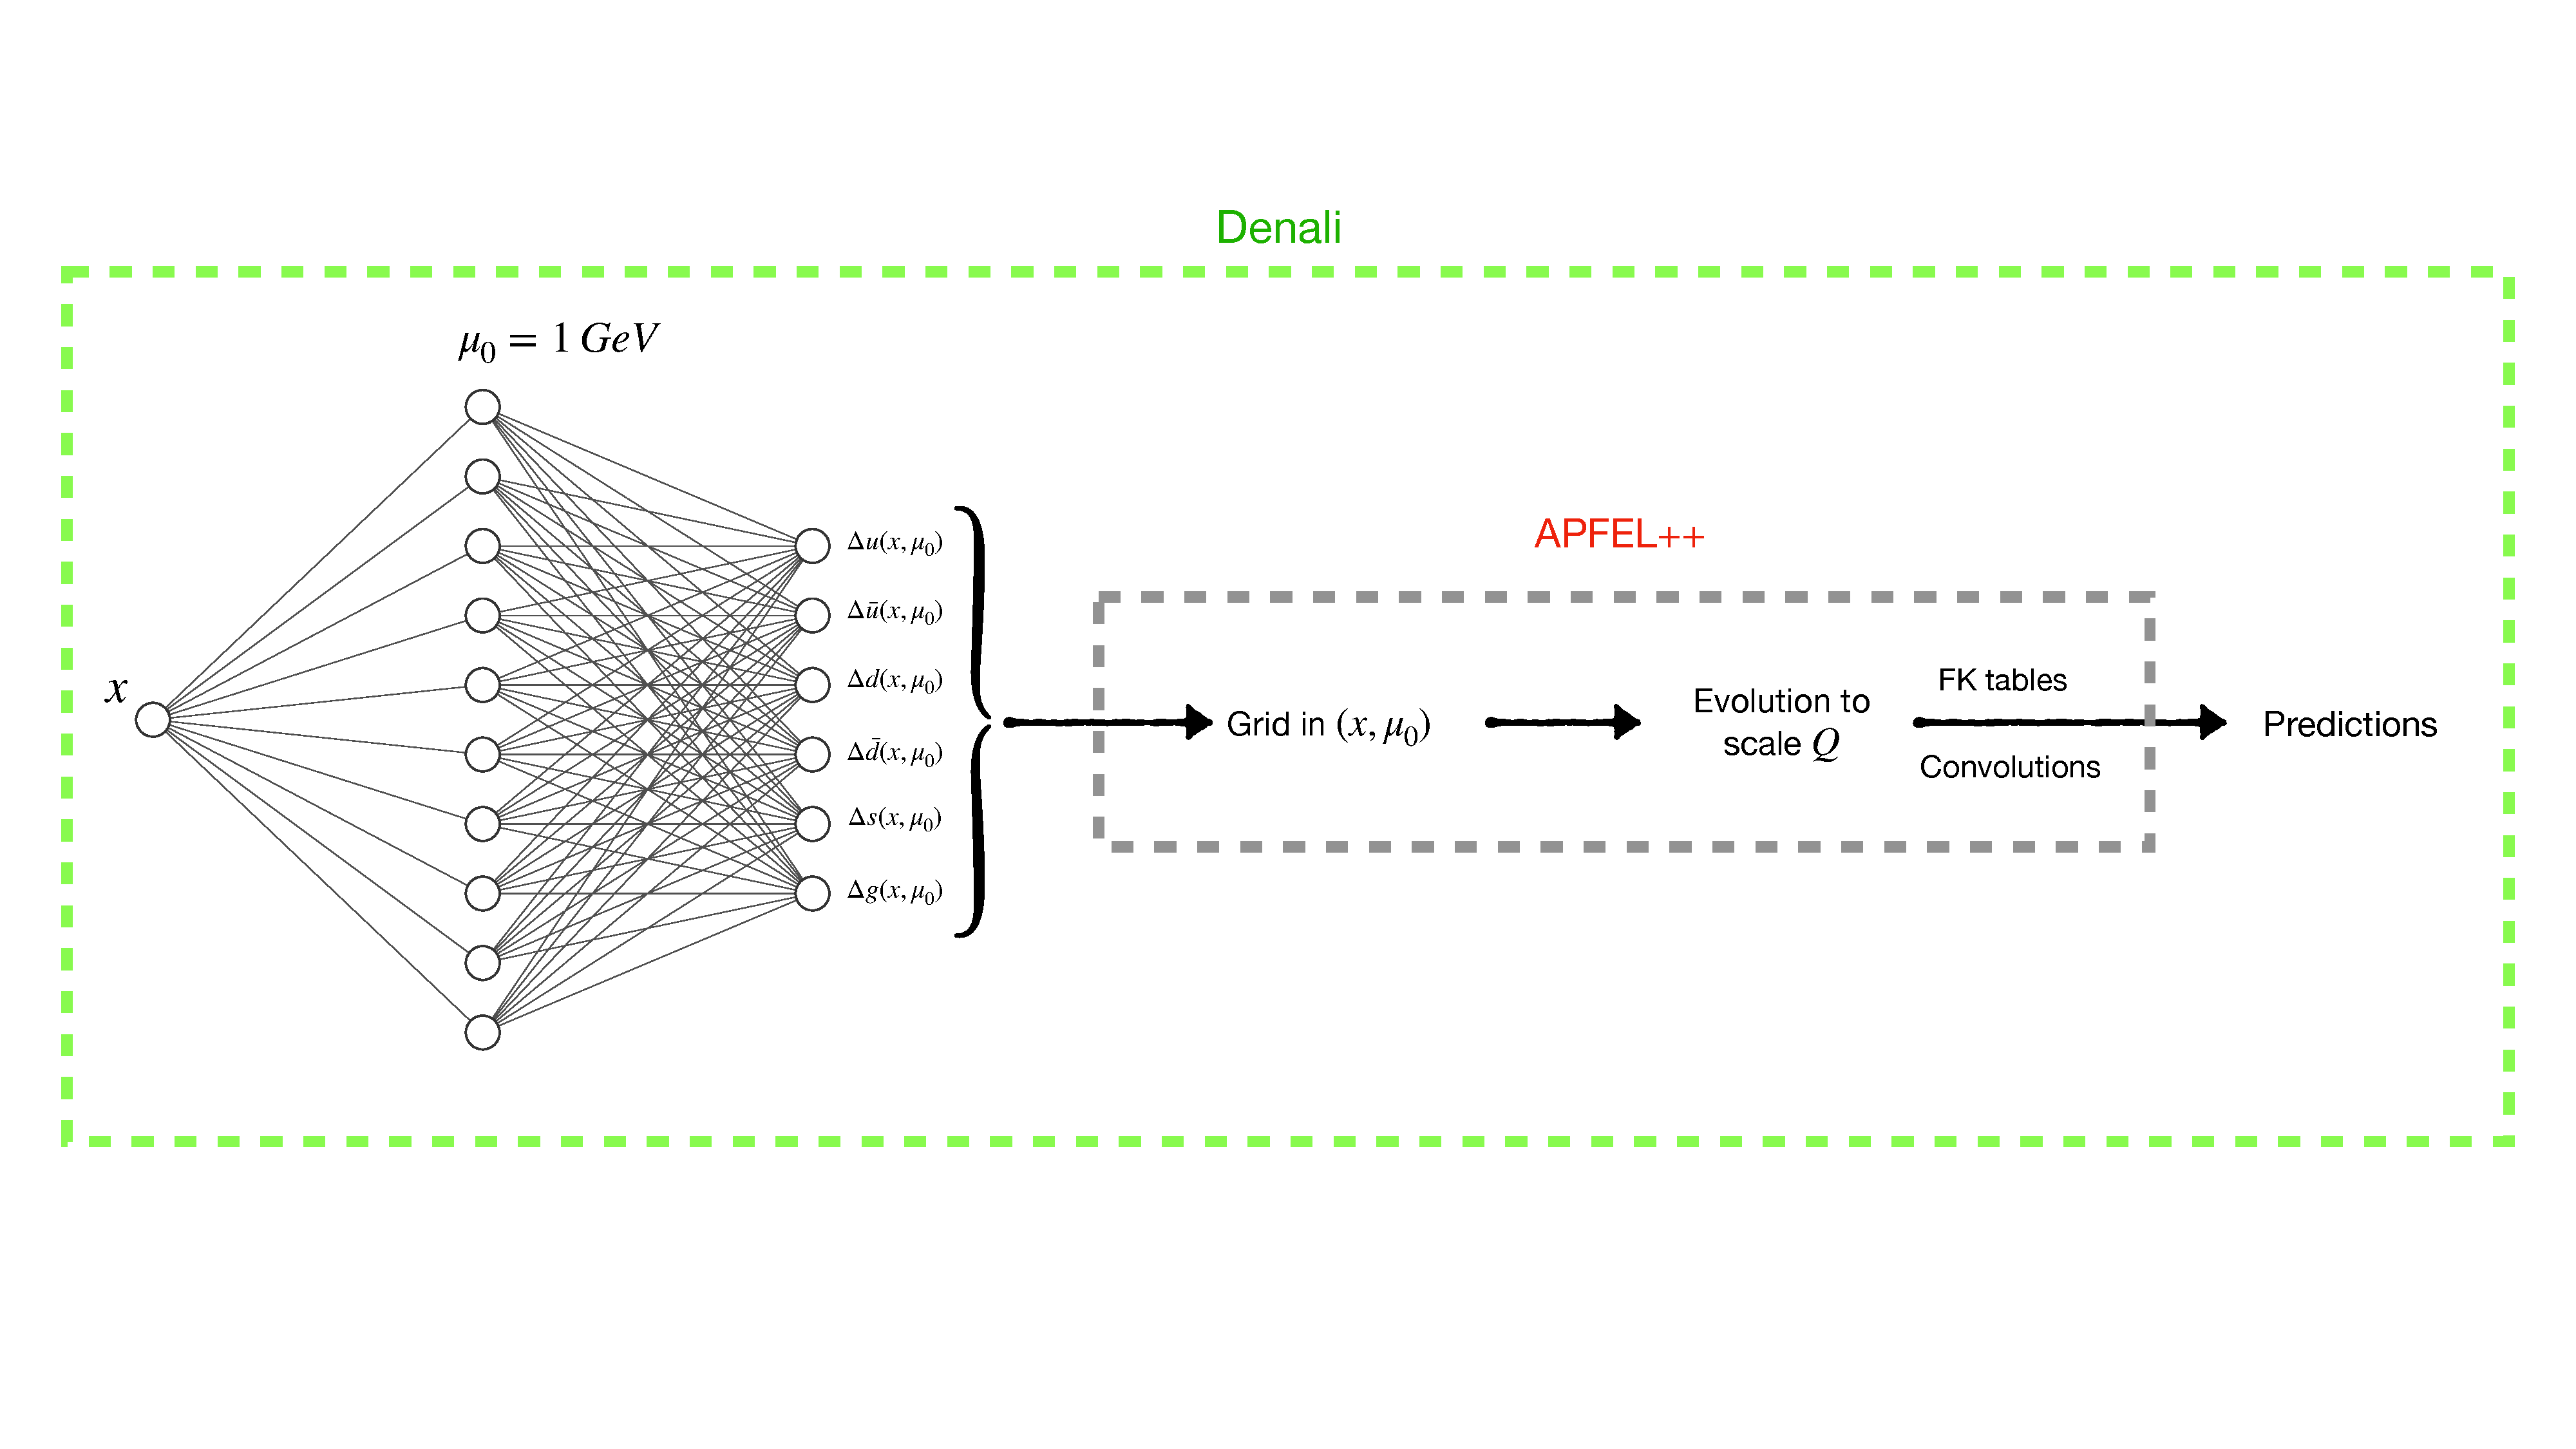
\includegraphics[width=1\textwidth]{NN_plot.pdf} 
  \caption{\small{Scheme of the \texttt{Denali} algorithm.}}
  \label{fig:NN_plot}
\end{figure}
%%

\subsection*{Optimization and determination of the optimal fit}
The process where the parameters are optimised over the parameter space through the minimisation of the figure of merit goes under the name of optimisation. Each replica of the PDF ensemble (\textit{i.e.}, each network) undergoes an independent optimisation procedure. Although this process can be computationally expensive if a high number of replicas is used, parallel processing methods can be exploited to considerably reduce the time required by a single global fit.%

The figure of merit for the $k$-th replica, minimised during the optimisation, is defined as
%%
\begin{equation}
  E^{(k)} = \frac{1}{N_{\T{dat}}} \sum_{i,j}^{N_{\T{dat}}} \left( F_{i}^{\T{(art)}(k)} - F_{i}^{\T{(net)}(k)} \right) (\T{cov})^{-1}_{ij} \left( F_{j}^{\T{(art)}(k)} - F_{j}^{\T{(net)}(k)} \right) \,.
  \label{eq:EF_k}
\end{equation}
%%
Here, $F_i$ may represent one of the observable presented in Tabs.~[\ref{tab:DIS_data},\ref{tab:SIDIS_data}]. 
The above expression requires few comments. The observable $F_{i}^{\T{(art)}(k)}$ is the $k$-th Monte Carlo replica of the $i$-th data point, whereas $F_{i}^{(net)(k)}$ is its prediction provided by the $k$-th neural network representing the corresponding replica of the PDF ensemble. Finally, $\T{(cov)}$ is the usual covariance matrix constructed from the experimental sets. The parameter space is explored with the SGD method discussed in \secref{sec:NNtr}, which sought for the minimum of the error function, Eq.~\eqref{eq:EF_k}.%

The error function, Eq.~\eqref{eq:EF_k}, must not be confused with the $\chi^2$ used to quantify the quality of the fit. Indeed, it can be shown that Eq.~\eqref{eq:EF_k} does converge to $2$ instead of $1$. The reason being that the prediction is compared against the fluctuated data and not against the experimental central value. Indeed, the statistical estimator that quantifies the fit quality is defined as
%%
\begin{equation}
  \chi^2 = \frac{1}{N_{\T{dat}}} \sum_{i,j}^{N_{\T{dat}}} \left( F_{i}^{\T{(exp)}} - \left<F_{i}^{\T{(net)}}\right>_{\T{rep}} \right) (\T{cov})^{-1}_{ij} \left( F_{j}^{\T{(exp)}} - \left<F_{j}^{\T{(net)}}\right>_{\T{rep}} \right) \,,
  \label{eq:global_chi2}
\end{equation}
%%
where $F_{i}^{\T{(exp)}}$ is the $i$-th experimental central value and the average over replicas is defined as
%%
\begin{equation}
  \left< F_i^{\T{(net)}} \right>_{\T{rep}} = \frac{1}{N_{\T{rep}}} \sum_{k} F^{(k)}_i \,.
\end{equation}
%%
I will refer to Eq.~\eqref{eq:global_chi2} as the global $\chi^2$ per data point, or simply $\chi^2$. It is computed at the end of the optimisation procedure and, thus, it is not minimised.%

As discussed at the end of \secref{sec:NNtr}, the neural network parametrisation is able to fit not only the underlying physics, but also statistical noise of the data set -- a problem also known as \textit{overlearning}. Thus, the best fit does not always coincide with the minimum of the figure of merit, Eq.~\eqref{eq:EF_k}. In order to find the best fit, the cross-validation method \cite{pml1Book} is implemented. It works as follows:
%%
\begin{enumerate}
  \item For each replica, the data sets are randomly divided into two sets -- training and validation sets. They include a fraction $f_{\T{tr}}$ and $f_{\T{val}} = 1 - f_{\T{tr}}$ of the data points, respectively.
  \item During the optimisation procedure, the error function, Eq.~\eqref{eq:EF_k}, is separately computed over the training and the validation set. The former undergoes the minimisation procedure, while the latter is only monitored and not minimised.
  \item Finally, the best fit corresponds to the minimum of the error function of the validation set within a fixed number of iterations, which in this case corresponds to $N_{\T{iter}} = 3000$.
\end{enumerate}
%%
The profile of the figure of merit for an arbitrary replica is shown in Fig.~\ref{fig:profile}. It is possible to see that, immediately after the minimum of the validation curve is reached, it starts to increase, whereas the training curve keeps reducing. This means that the network is learning the statistical noise of the training set, which is different from that of the validation set. In this analysis, equal training and validation fractions are chosen, that is $f_{\T{tr}} = f_{\T{val}} = 50\%$. However, some experimental sets are highly affected by the kinematic cuts and only a small portion of data points survives. In this case, the training set would be too small, affecting the stability of the minimisation. Hence, if the number of points after cuts is less or equal to 5, all the points will be included in the training set.

%%
\begin{figure}[t]
  \centering
  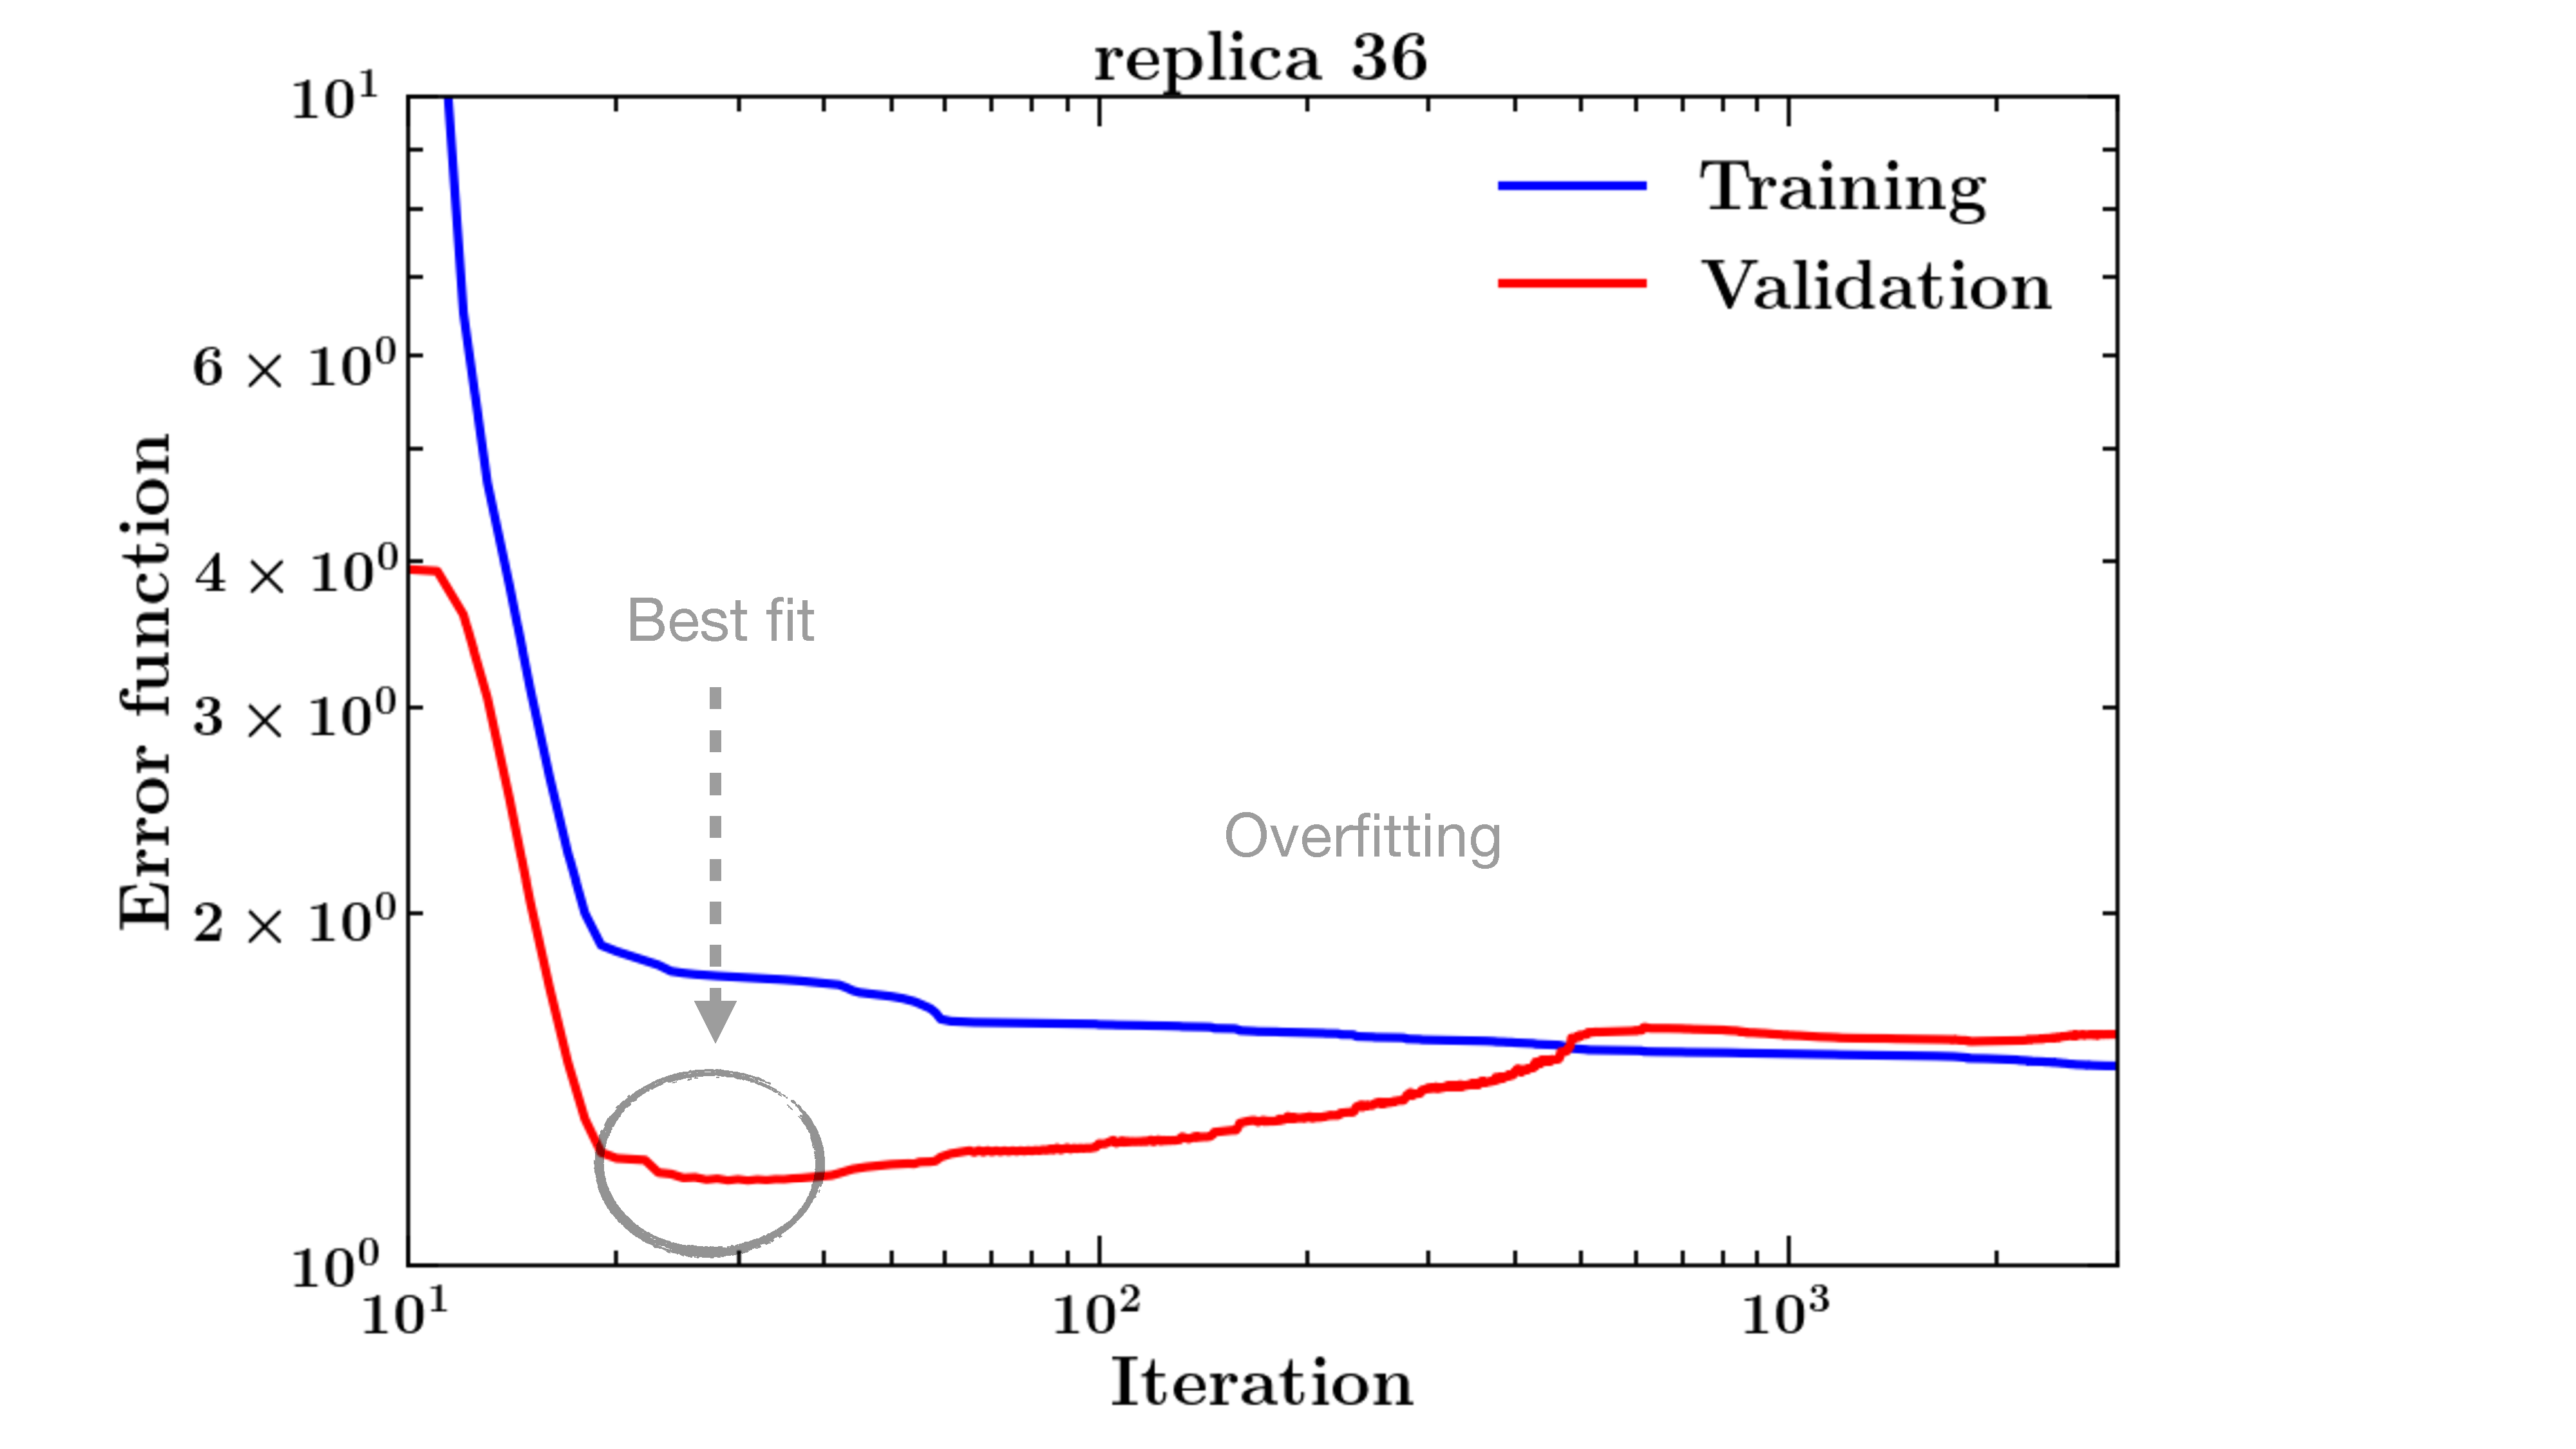
\includegraphics[width=0.6\textwidth]{profile.pdf} 
  \caption{\small{Profile of the error function for the 36th replica. The blue and red curves represent the error as a function of the iteration step for the training and validation sets, respectively.}}
  \label{fig:profile}
\end{figure}
%%

\subsection*{Theoretical constraints}
I have already mentioned that, due to the scarcity and the low accuracy of data, polarised PDFs are loosely constrained. This not only affects the efficiency of the algorithm, but has a huge impact on the fit quality. In order to improve the constraining power and to reduce the uncertainties of the polarised PDFs, I apply two theoretical constraints to the analysis -- sum rules and positivity.%

Sum rules refer to the hadronic matrix elements $a_3$ an $a_8$, whose values can be extracted from measurements in hyperon $\beta$-decay, Eqs.~\eqref{eq:a3_a8_values}. They can be related to the PDFs via Eqs.~(\ref{eq:a3_PM}-\ref{eq:a8_PM}), provided that exact $SU(3)_f$ symmetry is assumed. The theoretical constraint is introduced at data set level. This means that the values in \eqref{eq:a3_a8_values} are treated as standard data points, with central values and (uncorrelated) uncertainties. Hence, at each iteration of the optimisation procedure, the algorithm will compute, in addition to the observable $g_1^{(h)}$ or $g_1^{(h)}/F_1^{(h)}$, the predictions for $a_3$ and $a_8$ via Eqs.~(\ref{eq:a3_PM}-\ref{eq:a8_PM}). Sum rules provide further information on polarised PDFs. If the SIDIS data sets were not included, the only source of information for the sea-quark flavour $\Delta s$ would only come from this theoretical constraint.%

The other theoretical constraint is the positivity constraint. The key point is that the cross-sections that enter the polarised asymmetry, Eq.~\eqref{eq:asymmetry}, must be positive. This implies that $g_1^{(h)}$ is bounded by its unpolarised counterpart $F_1^{(h)}$, that is
%%
\begin{equation}
  \begin{split}
    \left| g_1 (x,Q^2)  \right|& \leq F_1(x, Q^2) \,,\\
    \left| g_1^{(h)} (x,z,Q^2)  \right|& \leq F_1^{(h)}(x, z, Q^2) \,.
  \end{split}
  \label{eq:positivity_obs}
\end{equation}
%%
Given that at leading order the structure function are proportional to parton distributions, and that Eq.~\eqref{eq:positivity_obs} must be satisfied for any choice of target (\textit{i.e.}, for any combination of quark plus antiquarks), it must be satisfied by each flavour separately. Hence, at leading order, the bound reads
%%
\begin{equation}
  \left| \Delta f_i (x,Q^2) \right| \leq f_i (x,Q^2) \,,
  \label{eq:positivity_fl}
\end{equation}
%%
for all $x$ and for all $Q^2$, being $f_i$ the relative unpolarised PDF set. At NLO and beyond the positivity constraint, Eq.~\eqref{eq:positivity_fl}, receives perturbative corrections. Nevertheless, it can be shown \cite{Altarelli:1998gn} that, even at relatively small values down to $Q^2 \sim 1 \, \T{Gev}^2$, the modified positivity bounds for each flavour are slightly modified, and the difference between LO and higher orders is negligible. Moreover, the positivity bound exhibits his constraining effects only at large $x$, where the higher order corrections to the LO positivity bound are lessened. Thus, imposing positivity bounds consistently guarantees positivity of physical cross-sections.%

The positivity bound Eq.~\eqref{eq:positivity_fl} must take into account the uncertainties of the unpolarised PDFs. This problem can be addressed with two different methods. The first imposes the leading-order bound, Eq.~\eqref{eq:positivity_fl}, by requiring
%%
\begin{equation}
  \left| \Delta f_i (x,Q^2) \right| \leq \left<f_i (x,Q^2)\right>_{\T{rep}} + \sigma_i(x,Q^2) \,,
  \label{eq:positivity_fl_sigma}
\end{equation}
%%
where $\left<f_i (x,Q^2)\right>_{\T{rep}}$ is the mean value over the statistical ensemble of unpolarised PDFs and $\sigma_i(x,Q^2)$ its corresponding one-sigma uncertainty, both evaluated at the kinematic point $(x,Q^2)$. This ensures that also the uncertainty of the unpolarised distribution is propagated through the analysis within the confidence level. The second approach applies the same bound Eq.~\eqref{eq:positivity_fl}, but with randomly chosen replica from the statistical set of distributions
%
\begin{equation}
  \left| \Delta f_i (x,Q^2) \right| \leq f_i^{(k)} (x,Q^2)\,, \hspace{4mm} k \hspace{2mm} \T{random}.
  \label{eq:positivity_random}
\end{equation}
%%
This means that the unpolarised PDF replica that enters the constraint is different for each polarised replica. This stocasticity spans the space of distributions, propagating the uncertainties of the unpolarised statistical ensemble through the bound. In both methods, consistency requires that the unpolarised parton set used to impose the positivity bound is the same that has been used to compute the unpolarised structure function $F_1^{(h)}$.%

The positivity constraint is introduced analytically, acting on the output layer of the neural network. Indeed, for each node of the last layer (\textit{i.e.}, for each parametrised flavour), I impose
%%
\begin{equation}
  \sigma_{i} (x,\mu_0) \rightarrow \Delta f_{i} (x, \mu_0) \equiv \bigl[ 2 \sigma(x,\mu_0) - 1 \bigr] \, f_{i} (x,\mu_0) \,,
  \label{eq:pos_net}
\end{equation}
%%
being $\sigma_i(x,\mu^2_0)$ the sigmoid activation function of the $i$-th output of the network. We observe that Eq.~\eqref{eq:pos_net} not only imposes the positivity bound Eq.~\eqref{eq:positivity_fl}, but also constraint to zero parton distribution at $x=1$, provided that the unpolarised PDF is zero at the same point. 

%%%%%%%%%%%%%%%%%%%%%%%%%%%%%%%%%%%%%%%%%%%%%%%%%%%%%%
\section{Results}
\label{sec:4.4}

I present the first determination of polarised PDFs \texttt{MAPpol1.0} obtained at next-to-next-to-leading order accuracy. It relies on the methodologies that have been covered earlier and includes the data sets introduced in \secref{sec:4.1}. The parton distributions have been parametrised at an initial scale $\mu_0 = 1\,\T{Gev}$, below the heavy quark mass thresholds. Hence, the contribution of heavy quarks has been neglected, and the corresponding distributions have been set to zero. Throughout the QCD analysis, mass corrections have also been neglected. The unpolarised set of PDFs used to compute the unpolarised structure functions $F_1^{(h)}$ and to impose the positivity constraint is \texttt{NNPDF31\_nnlo\_pch\_as\_0118}~\cite{NNPDF:2017mvq}, while the set of FFs necessary to compute the SIDIS observables is \texttt{MAPFF1.0}~\cite{Khalek:2021gxf, AbdulKhalek:2022laj}. This fitting configuration, which is summarised in Tab.~\ref{tab:baseline}, represents the default set-up, and I will refer to it as the \textit{baseline} configuration.%

First, I present the \texttt{MAPpol1.0} set and its statistical features. The impact of higher order corrections is discussed and compared with the NLO determination obtained with the same fitting configuration. Then, I compare the \texttt{MAPpol1.0} set with other available sets, focusing out the main differences that arise among them. Finally, I review the effects of the theoretical constraints and assess the stability of the results by performing a number of variations w.r.t. the baseline setting.

\begin{table}[b!]
  \centering 
  \small
  \begin{tabular}{l@{\hspace{1cm}}c}
  \toprule \midrule
  \addlinespace
      Experiment        &   Baseline \texttt{MAPpol1.0}        \tabularnewline
  \midrule
  \addlinespace
      Parametrised PDFs & $\Delta u,\,\Delta d,\,\Delta s,\,\Delta\bar{u},\,\Delta\bar{d}$ and $\Delta g$         \tabularnewline
      \midrule
      \addlinespace
      Unpolarised PDFs set  &  \texttt{NNPDF31\_nnlo\_pch\_as\_0118}~\cite{NNPDF:2017mvq}   \tabularnewline
      \midrule
      \addlinespace
      FFs set               &  \texttt{MAPFF1.0}~\cite{Khalek:2021gxf, AbdulKhalek:2022laj} \tabularnewline
      \midrule
      \addlinespace
      Positivity            &  $\left| \Delta f_i  \right| \leq f_i^{(k)}$ , $k$ random                \tabularnewline
      \midrule
      \addlinespace
      Sum rules             &   $a_3$ and $a_8$                                             \tabularnewline
      \midrule
      \addlinespace
      Number of replicas    &               150                                             \tabularnewline
      \midrule
      \addlinespace
      NN architecture       &   $(1,10,6)$                                                  \tabularnewline
  \midrule \bottomrule
\end{tabular}
  \caption{
    \small
    Fitting configuration of baseline setting of the \texttt{MAPpol1.0} set.
  \label{tab:baseline}}
\end{table}

\begin{figure}[t!]
  \centering
  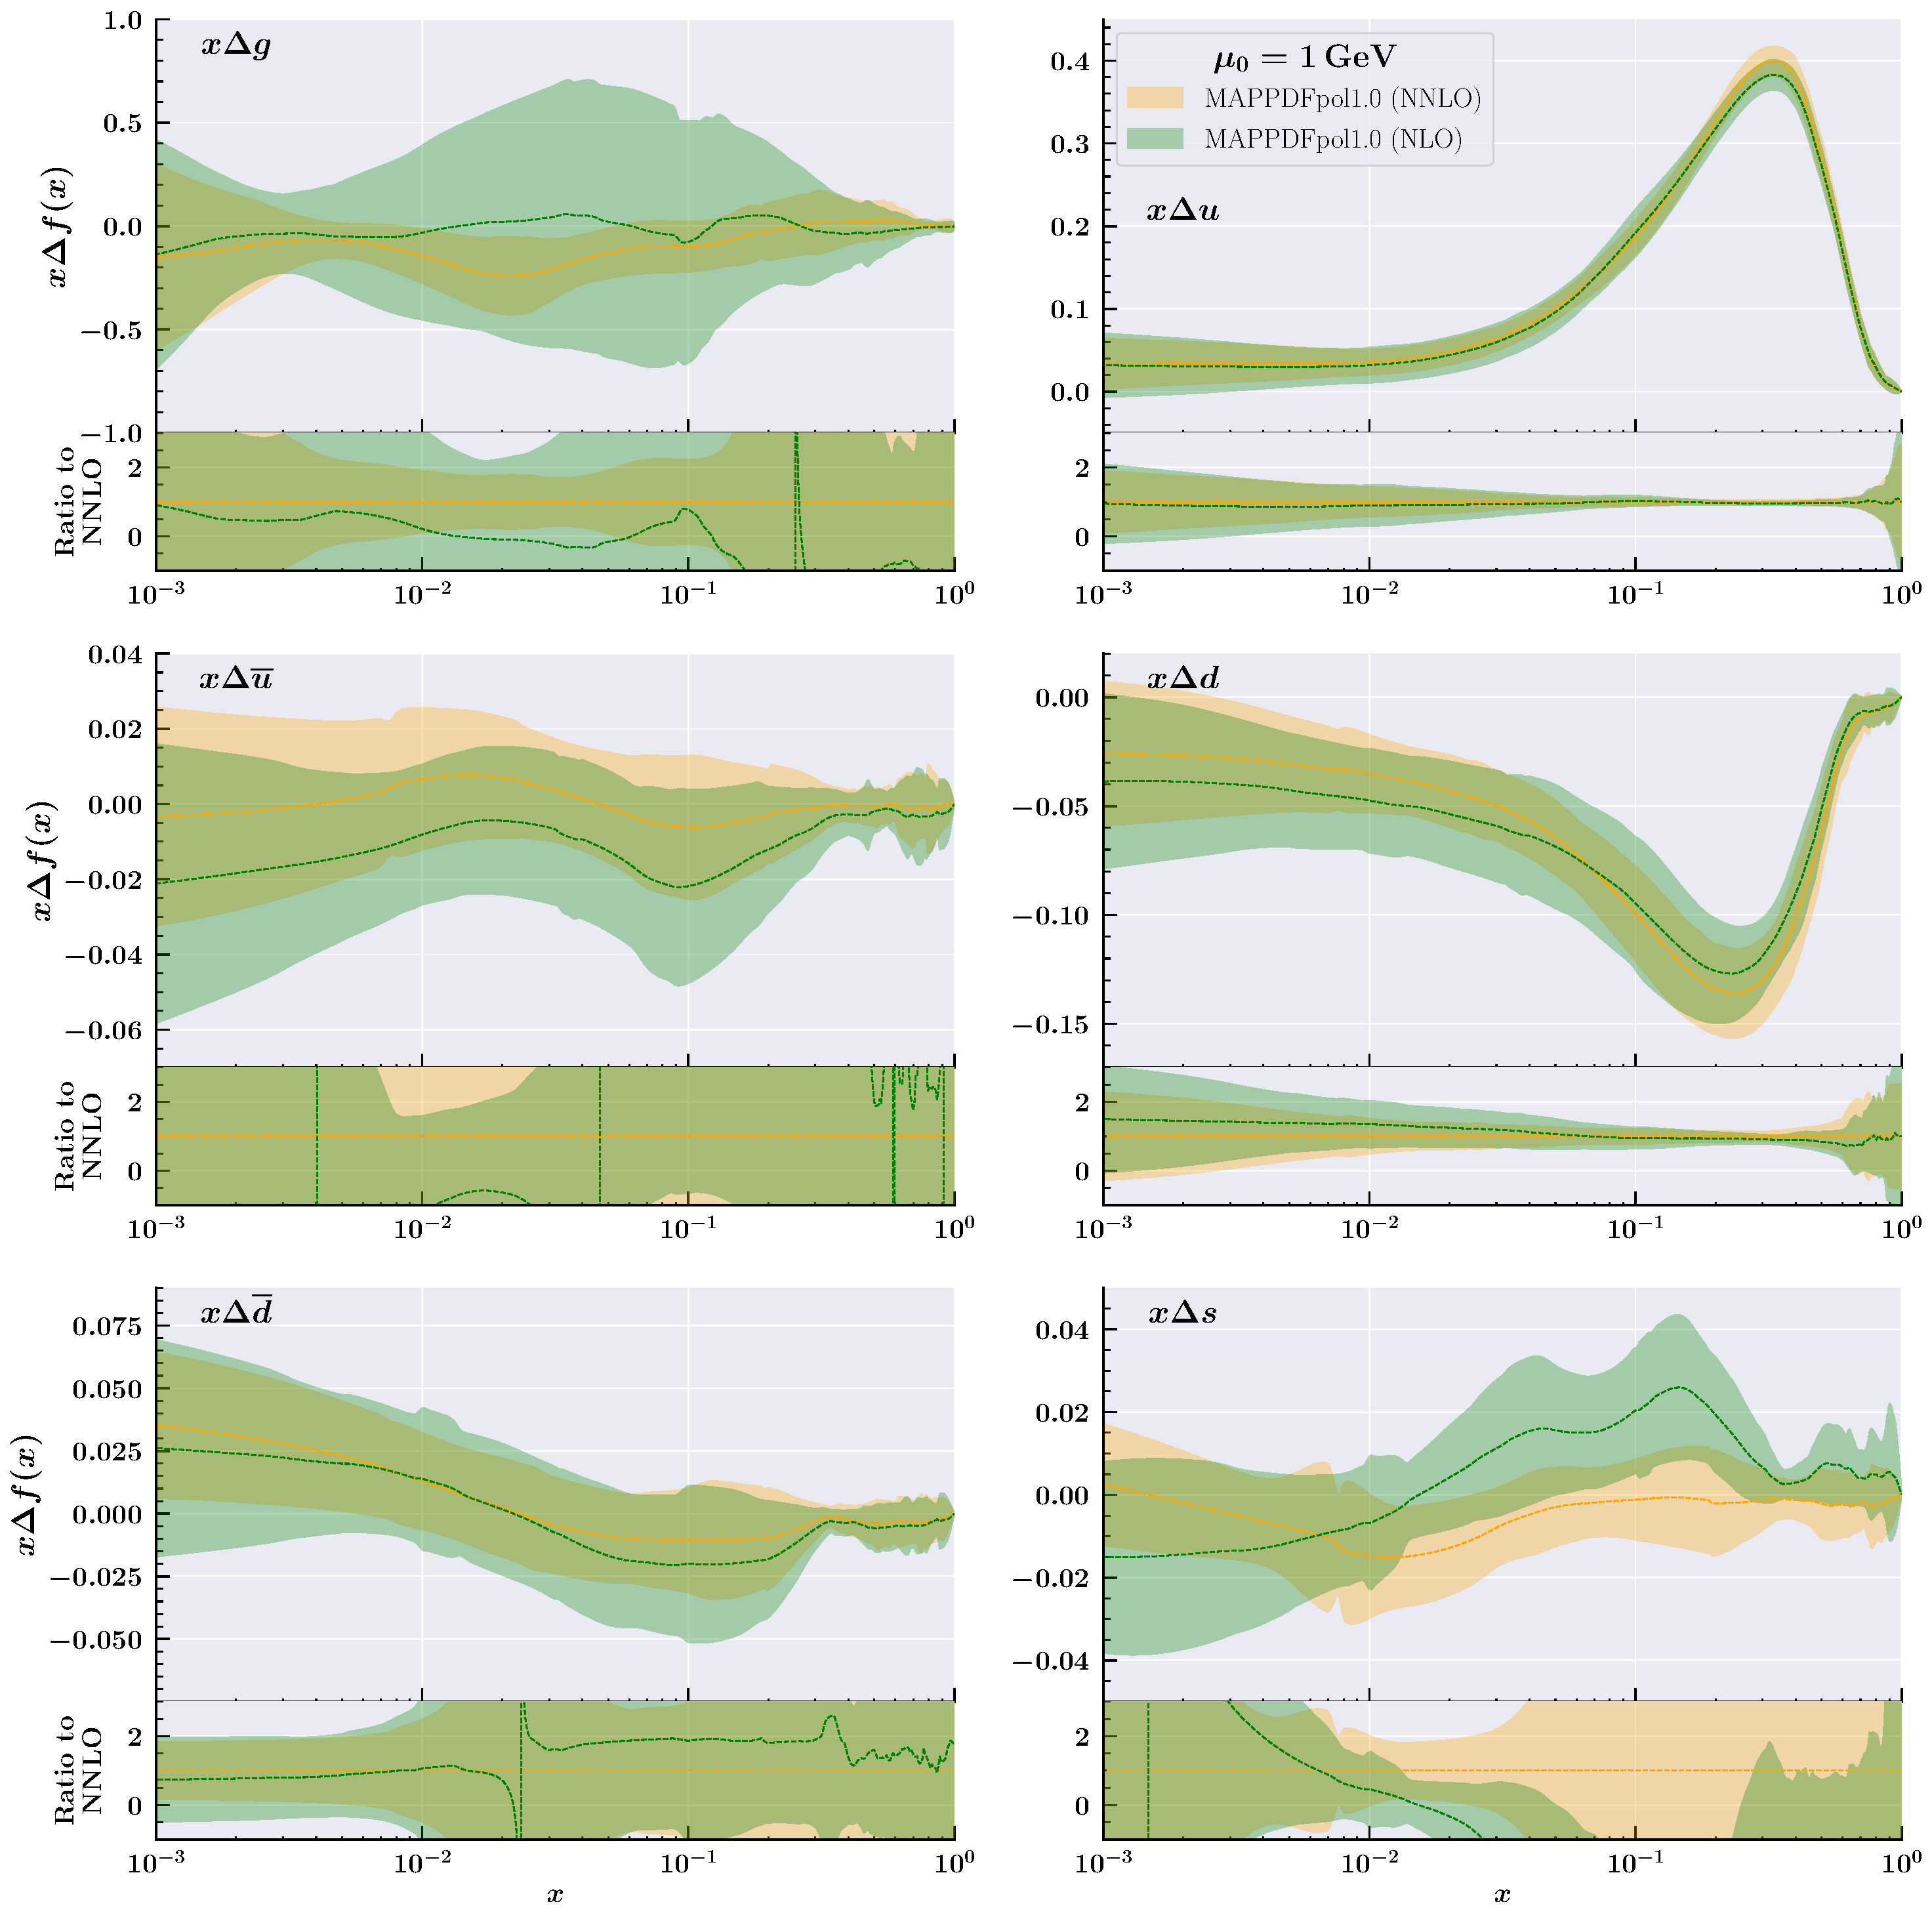
\includegraphics[width=\textwidth]{Chapters/Chapter_4/figs/nnlo_nlo_ratio.pdf}
  \caption{\small Comparison between the NNLO and NLO \texttt{MAPpol1.0} sets at $\mu_0 = 1 \, \T{GeV}$ in flavour basis and plotted as functions of $x$. For each flavour, the absolute values of the distributions are displayed in the upper panel and their ratio to the central value of the NNLO fit in the lower one.}
  \label{fig:nnlo_nlo}
\end{figure}

%_______________________________________
\subsection{Impact of NNLO corrections}

\begin{table}[t!]
  \centering % Center table
  \small
  \begin{tabular}{l@{\hspace{1cm}}c@{\hspace{1cm}}c@{\hspace{1cm}}c}
  \toprule \midrule
  \addlinespace
                        &  $N_{\T{dat}}$  & \multicolumn{2}{c}{$\chi^2/N_{\T{dat}}$} \\
  \cmidrule(lr){3-4}
      Experiment        &           &   \texttt{MAPpol1.0} (NLO)   &  \texttt{MAPpol1.0} (NNLO)  \tabularnewline
  %\cmidrule[\lightrulewidth](lr){1-3}\addlinespace[1ex]
  \midrule
  \addlinespace
      COMPASS-P $K^-$  &  12 &   0.73   &   0.95   \tabularnewline
      COMPASS-P $K^+$  &  12 &   0.73   &   0.93   \tabularnewline
    COMPASS-P $\pi^-$  &  12 &   1.36   &   1.19   \tabularnewline
    COMPASS-P $\pi^+$  &  12 &   2.31   &   1.99   \tabularnewline
      COMPASS-D $K^-$  &  10 &   0.97   &   0.77   \tabularnewline
      COMPASS-D $K^+$  &  10 &   0.32   &   0.36   \tabularnewline
    COMPASS-D $\pi^-$  &  10 &   0.51   &   1.44   \tabularnewline
    COMPASS-D $\pi^+$  &  10 &   0.30   &   1.21   \tabularnewline
      HERMES-D  $K^-$  &   9 &   0.65   &   1.06   \tabularnewline
      HERMES-D  $K^+$  &   9 &   1.49   &   1.71   \tabularnewline
    HERMES-D  $\pi^-$  &   9 &   1.37   &   2.29   \tabularnewline
    HERMES-D  $\pi^+$  &   9 &   0.33   &   1.41   \tabularnewline
    HERMES-P  $\pi^-$  &   9 &   1.04   &   0.68   \tabularnewline
    HERMES-P  $\pi^+$  &   9 &   1.89   &   1.91   \tabularnewline
               E142-N  &   7 &   0.60   &   0.80   \tabularnewline
               E143-D  &  25 &   1.30   &   1.24   \tabularnewline
               E143-P  &  25 &   0.73   &   0.70   \tabularnewline
               E154-N  &  11 &   0.23   &   0.19   \tabularnewline
               E155-P  &  22 &   0.66   &   0.79   \tabularnewline
               E155-N  &  22 &   0.71   &   0.82   \tabularnewline
                EMC-P  &  10 &   0.58   &   0.53   \tabularnewline
         JLAB E06 014  &   1 &   0.69   &   0.90   \tabularnewline
         JLAB E97 103  &   0 &   0.00   &   0.00   \tabularnewline
         JLAB E99 117  &   0 &   0.00   &   0.00   \tabularnewline
      JLAB EG1 DVCS-D  &   1 &   0.00   &   0.00   \tabularnewline
      JLAB EG1 DVCS-P  &   2 &   0.00   &   0.00   \tabularnewline
                SMC-D  &  12 &   1.33   &   1.17   \tabularnewline
                SMC-P  &  12 &   0.28   &   0.29   \tabularnewline
            COMPASS-D  &  15 &   0.35   &   1.02   \tabularnewline    
            COMPASS-P  &  17 &   0.59   &   0.80   \tabularnewline
             HERMES-N  &   8 &   0.22   &   0.26   \tabularnewline
             HERMES-D  &  14 &   0.66   &   0.67   \tabularnewline
             HERMES-P  &  14 &   0.45   &   0.45   \tabularnewline
       $a_3$ sum rule  &   1 &   0.25   &   0.51   \tabularnewline
       $a_8$ sum rule  &   1 &   0.00   &   0.02   \tabularnewline
  \midrule
  \addlinespace
                Total  & 362 &   0.64     &   0.75   \tabularnewline
  \midrule \bottomrule
\end{tabular}

  \caption{
    \small
    Values of the $\chi^2$ per data point computed with Eq.~\eqref{eq:global_chi2} for the individual data sets included in the \texttt{MAPpol1.0} analysis for NNLO and NLO distributions. The global $\chi^2$ values are also displayed.  
  \label{tab:nnlo_nlo_chi2}}% Add 'table' caption
\end{table}
%
The NNLO and NLO determinations obtained with the baseline set-up are presented in Fig.~\ref{fig:nnlo_nlo}. The values of the $\chi^2$ per data point computed with Eq.~\eqref{eq:global_chi2} are displayed in Tab.~\ref{tab:nnlo_nlo_chi2} for each data set included in the analysis. The values of the global $\chi^2$ per data point for the determinations at NLO and NNLO are also shown, and they are $0.68$ and $0.86$, respectively. This indicates a general good description of the entire data set for both fits. A closer inspection of Tab.~\ref{tab:nnlo_nlo_chi2} reveals that a good description is achieved for all individual data sets. In the case of JLAB data, the smallness of the $\chi^2$ is due to the fact that only a very small number of experimental points survives the kinematic cut (see Tab.~\ref{tab:DIS_data}), and hence it is not statistically significant. The discrepancy between the two values of the $\chi^2$ at NLO and NNLO seems to indicate that the global agreement between data and the central replica is worse for the NNLO case. However, the latter receives a significant enhancement in terms of accuracy of parton distributions, which balances the deterioration of the $\chi^2$.%

In the case of the gluon distribution $\Delta g$, the differences are mostly in terms of accuracy. On the one hand, the uncertainty is considerably smaller for the NNLO fit, in particular in the region $0.003 \lesssim x \lesssim 0.5$. On the other hand, the central value remains almost stable, except for the middle-$x$ region. However, it must be remarked that the gluon distribution remains poorly constrained by data, and the inclusion of difference processes other than those included in this analysis may considerably change the behaviour of the gluon.%

The impact of NNLO corrections on valence quark distributions $\Delta u$ and $\Delta d$ is moderate. In particular, the $\Delta u$ distributions are in perfect agreement in terms of both precision and accuracy. In the case of $\Delta d$, the central value receives a small upward shift at NNLO in the small-$x$ region, whereas the uncertainty slightly decreases in the middle-$x$ region.%

The sea-antiquark distributions $\Delta \bar{u}$ and $\Delta \bar{d}$ are generally affected by smaller uncertainties for the NNLO case. The central value $\Delta \bar{u}$ receives a small upward shift at NNLO, whereas the central value of $\Delta \bar{d}$ is almost unchanged.%

The major differences are observed in the case of the strange distribution $\Delta s$. The NNLO fit introduces a remarkable downward shift for the central value of the distribution in the central-$x$ region, restoring a behaviour which is similar to the LO. Also in this case, the uncertainty generally reduces, in particular in the small to medium-$x$ region.%

In conclusion, the impact of perturbative corrections is generally moderate, except for $\Delta g$ and $\Delta s$. The former presents a remarkable uncertainty reduction, while the latter is moved close to the behaviour at LO. The other distributions receive small enhancements in terms of accuracy, and the central values remain almost comparable between the two perturbative orders.
%The higher value of the global $\chi^2$ at NNLO can be ascribed to the fact that the analysis makes use of assumption $\Delta s = \Delta \bar{s}$. If true, this would indicate that NNLO corrections bear different information for $\Delta s$ and $\Delta \bar{s}$ separately. Hence, further studies should be carried out by relaxing this assumption and assessing the impact of independent parametrisations of the strange distributions.

%_______________________________________
\subsection*{Comparison with other PDF sets}

In Fig.~\ref{fig:competitors} I compared the PDFs obtained at NNLO from the baseline fit, \texttt{MAPpol1.0}, to other available PDF sets from \texttt{NNPDFpol1.1}~\cite{Nocera:2014gqa}, \texttt{JAM17}~\cite{Ethier:2017zbq} and \texttt{DSSV}~\cite{deFlorian:2008mr}. Here I present a brief summary of the main features that characterise each of these sets:
%%
\begin{itemize}
  \item[] \texttt{\textbf{NNPDFpol1.1}} The parton set is obtained using inclusive DIS data. Other experimental information coming from open-charm production in fixed-target DIS, and jet and $W$ production in proton-proton collisions are then included in the PDF ensemble via Bayesian reweighting and unweighting \cite{Ball:2011gg, Ball:2010gb}. The functional parametrisation is given by a set of neural networks, one for each parametrised distribution. The architecture is wider than that presented in this Thesis, with two deep-layers inside. Moreover, the parametrisation is supplied with two preprocessing functions accounting for the small- and large-$x$ behaviours. The uncertainties are estimated with the Monte Carlo sampling method. On the side of theoretical assumptions, this set imposes positivity \eqref{eq:positivity_fl} and sum rules \ref{eq:a3_a8_values} during the minimisation procedure through Lagrange multipliers. 
  \item[] \texttt{\textbf{JAM17}} This set uses data from inclusive and semi-inclusive DIS, together with single-inclusive $e^+ e^-$ annihilation data. This set is obtained by performing a simultaneous fit of both PDFs and FFs. Both are parametrised in terms of a polynomial function adjusted to account for the behaviours of the distributions. This set does not include positivity nor assumptions about $SU(3)$ symmetry. Also in this, case the uncertainties have been estimated by means of Monte Carlo sampling.
  \item[] \texttt{\textbf{DSSV}} The set takes into account data from inclusive and semi-inclusive polarised DIS, as well as from polarised $pp$ scattering at RHIC. These include prompt-photon production $pp \rightarrow \gamma X$, jet production $pp \rightarrow \T{jets} + X$, and heavy flavours production $pp -\rightarrow c\bar{c}X, \, b\bar{b}X, \, J/\psi X$. The parametrisation is given by a flexible functional form given by a polynomial. Two more free parameters are used to account for deviations from the assumption of exact $SU(2)$ and $SU(3)$ symmetries. No positivity bounds are imposed to parton distributions. The estimate of the uncertainties is based on the use of Lagrange multipliers, as described in Ref.~\cite{Stump:2001gu}.
\end{itemize}
%%
It must be observed that the above sets have been determined at NLO accuracy. The main observations coming from the inspection of Fig.~\ref{fig:competitors} are summarised below:
%%
\begin{figure}[t!]
  \centering
  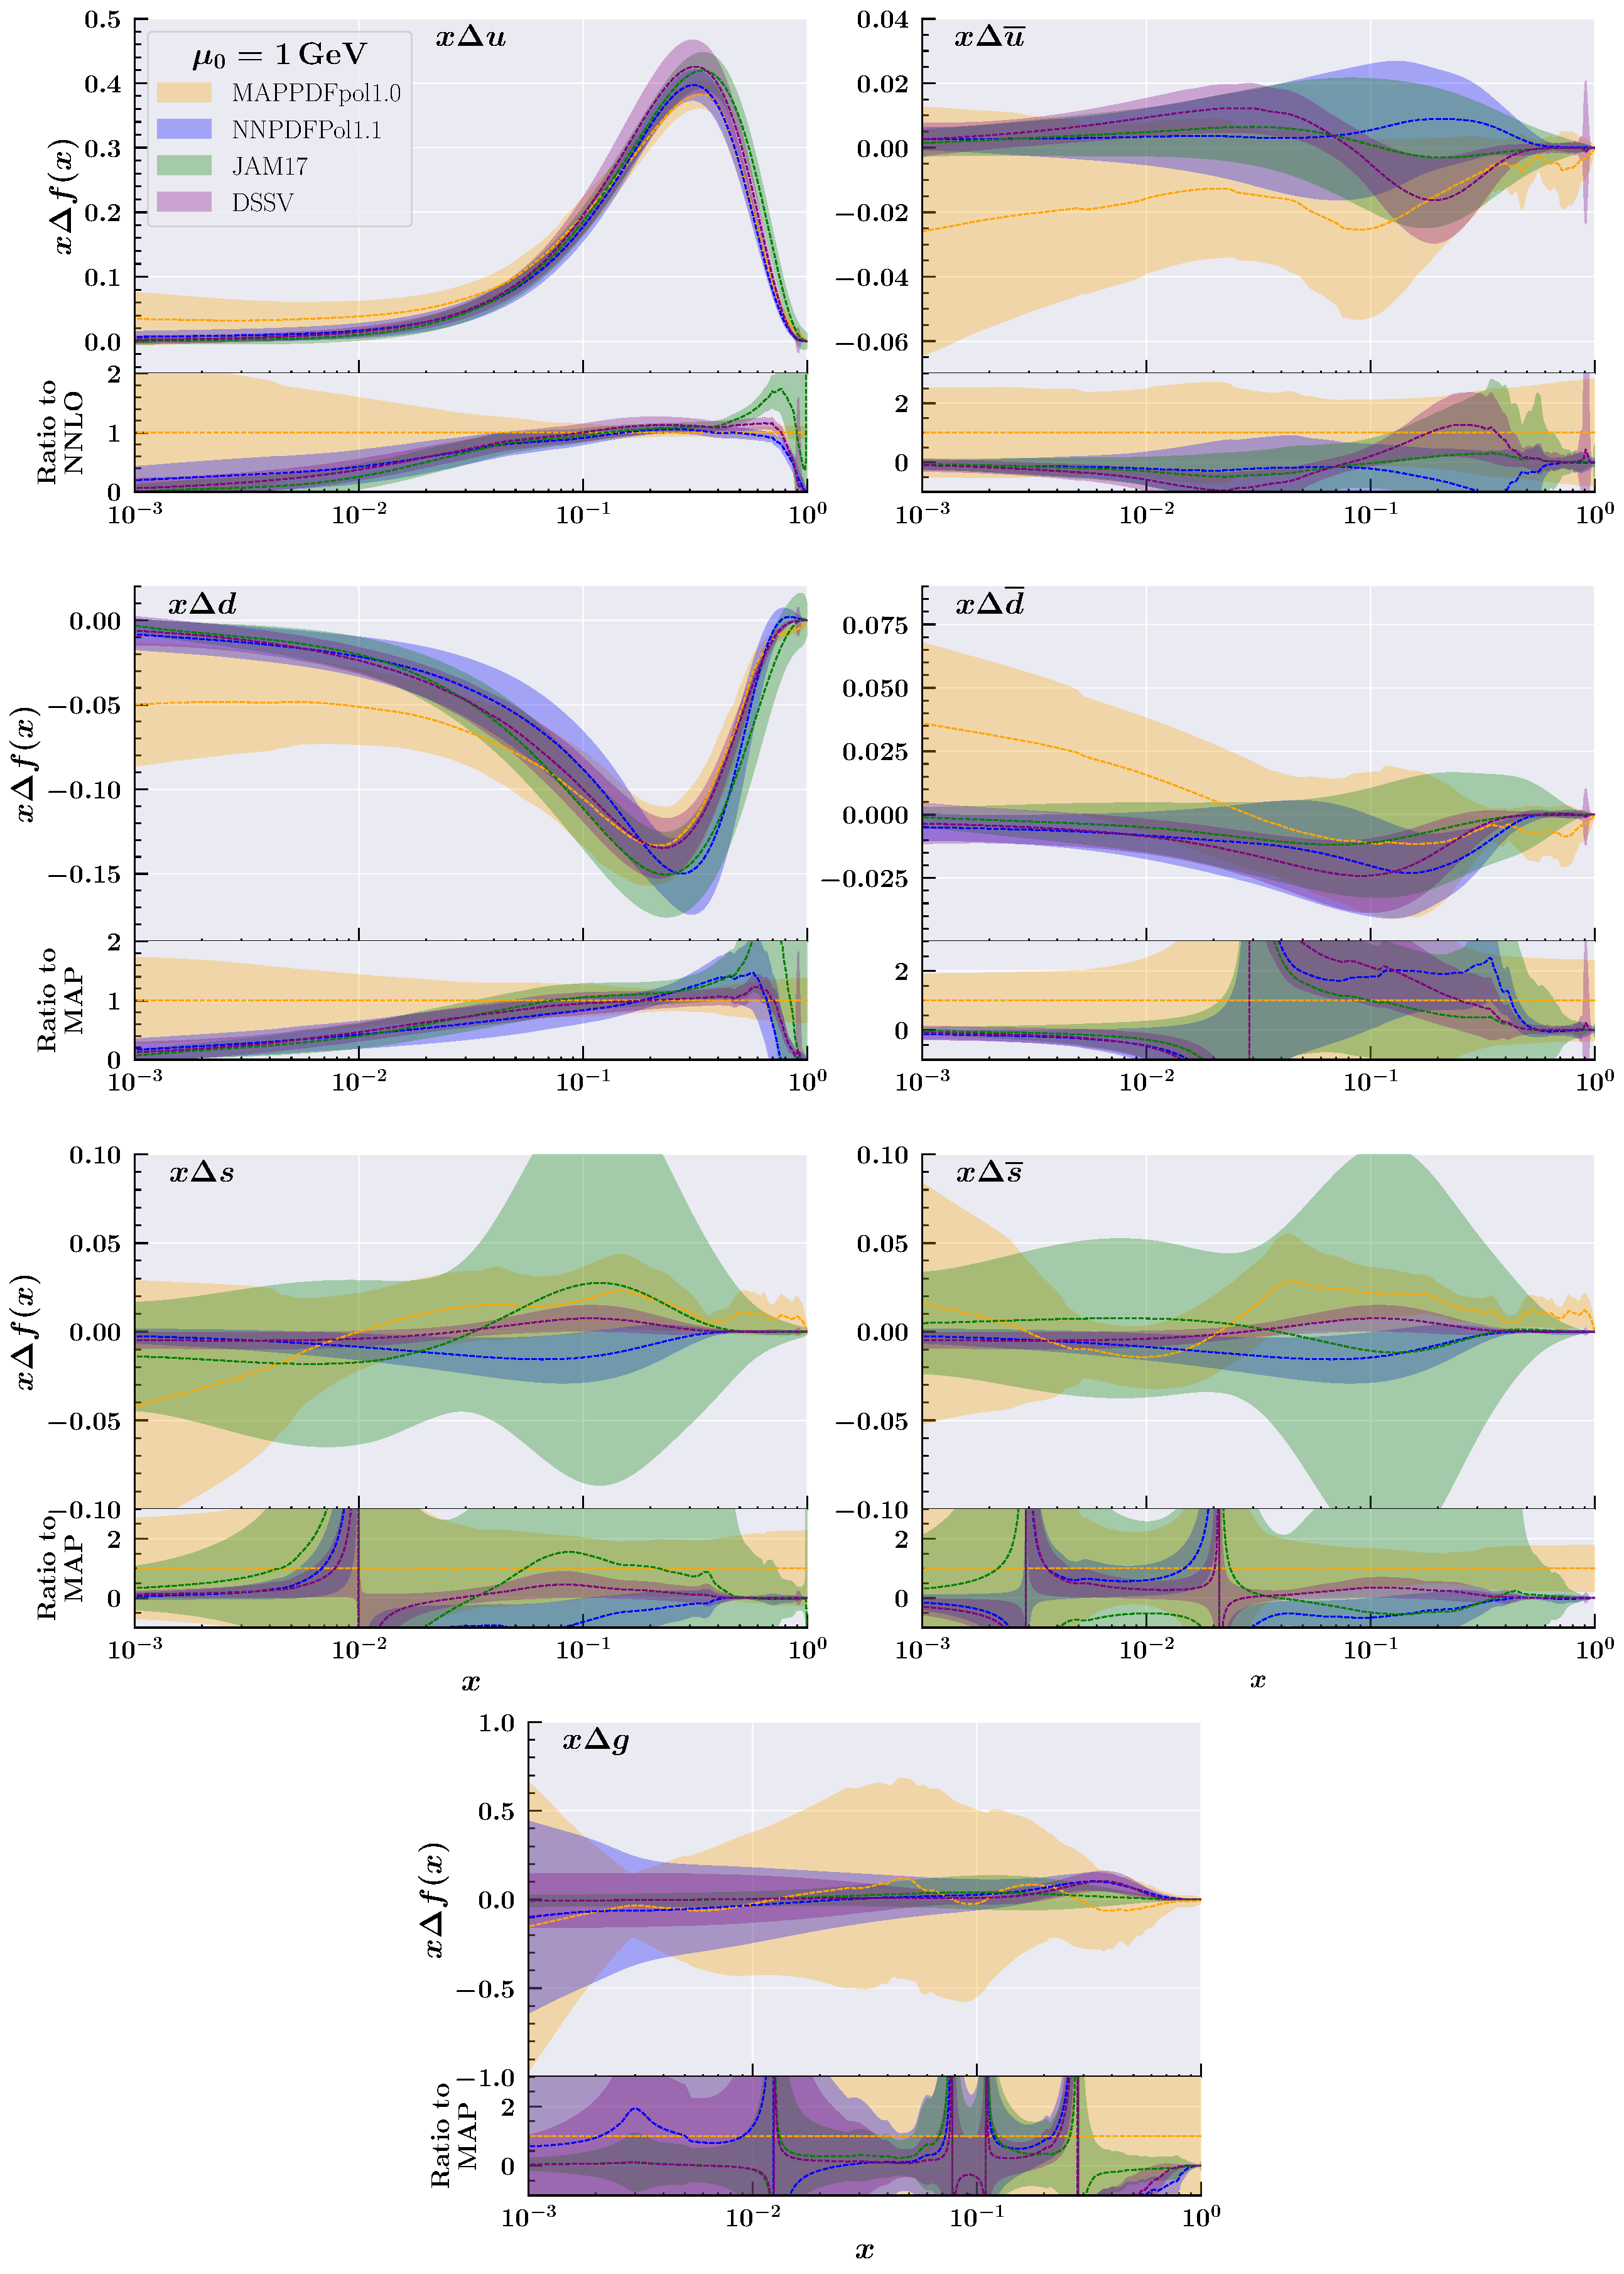
\includegraphics[width=\textwidth]{Chapters/Chapter_4/figs/competitors.pdf}
  \caption{\small{Comparison of the \texttt{MAPpol1.0}, \texttt{NNPDFpol1.1}~\cite{Nocera:2014gqa}, \texttt{JAM17}~\cite{Ethier:2017zbq} and \texttt{DSSV}~\cite{deFlorian:2008mr} sets. The distributions are displayed at $\mu_0 = 1 \, \T{GeV}$ in flavour basis. }}
  \label{fig:competitors}
\end{figure}
%
\begin{itemize}
  \item In the case of $\Delta g$, it is clear that the inclusion of gluon initiated-processes has a remarkable impact on the the final results, as the determinations from \texttt{NNPDFpol1.1} and \texttt{DSSV} show. Indeed, these distributions are in highly agreement between them, although the former provides a more conservative uncertainty estimate for $x \lesssim 0.1$. The lack of jet production data in \texttt{MAPpol1.0} is more evident in the middle-$x$ region, where the behaviour of the gluon slightly changes if compared to \texttt{NNPDFpol1.1} and \texttt{DSSV}. Nevertheless, both are within the \texttt{MAPpol1.0} uncertainties. The same does not hold for the gluon from \texttt{JAM17}, whose differences in the middle-$x$ region are not contained in the \texttt{MAPpol1.0} bounds. However, the agreement is then restored in the large-$x$ region, where \texttt{MAPpol1.0} is in broad agreement with the other sets.
  \item The valence quark distributions $\Delta u$ and $\Delta d$ from \texttt{MAPpol1.0} are in very good agreement with the corresponding distributions from the other available sets. For $x \lesssim 0.01$, where experimental data is sparse (see Fig.~\ref{fig:kin_cov}), the relative uncertainty on both $\Delta u$ and $\Delta d$ distributions from \texttt{MAPpol1.0} is larger than that of the corresponding distributions from \texttt{NNPDFpol1.0}, \texttt{JAM17} and \texttt{DSSV}. On the other hand, at large-$x$ the uncertainty reduces and becomes comparable to that of the other PDF sets.
  \item In the case of $\Delta \bar{u}$ and $\Delta \bar{d}$ distributions there is a good agreement at large $x$ with all the other determinations. In general, the \texttt{MAPpol1.0} is affected by a larger uncertainty, especially for $x \lesssim 0.01$, where DIS and SIDIS data is scarce. This is a consequence of the fact that \texttt{MAPpol1.0} does not include data from proton-proton collisions, whereas \texttt{DSSV} and \texttt{NNPDFpol1.1} do. Hence, their distributions have generally smaller uncertainties in this region thanks to $pp$ processes (\textit{e.g.} Drell-Yan or $W$ production), which provide more information on quark-antiquark pairs. On the other hand, the distributions from \texttt{JAM17}, which does not include proton-proton collisions nor SIDIS data either, are affected by smaller uncertainties than \texttt{MAPpol1.0}, maybe due to the simultaneous determination of PDFs and FFs.
  \item The $\Delta s$ distribution from \texttt{MAPpol1.0} receives its major contribution from SIDIS data and the axial moment $a_8$. Both \texttt{NNPDFpol1.1} and \texttt{DSSV} determinations include data from $pp$ collisions, but only the former exploits $SU(3)_f$ exact symmetry and introduces $a_8$ as a constraint. This difference may be the cause of the discrepancy that is observed between \texttt{NNPDFpol1.1} and \texttt{DSSV}, which is not included in the relative uncertainty bounds. Nevertheless, the \texttt{MAPpol1.0} determination is compatible with both of them. On the other hand, the uncertainty of \texttt{JAM17} is much more conservative than the uncertainties of the corresponding distributions from \texttt{MAPpol1.0}, \texttt{NNPDFpol1.1} and \texttt{DSSV}, maybe due to the lack of SIDIS data.
\end{itemize}
%%

%%%%%%%%%%%%%%%%%%%%%%%%%%%%%%%%%%%%%%%%%%%%%%%
\subsection{Impact of theoretical assumptions}
The results presented in this Thesis have been obtained with a number of theoretical and methodological constraints, as discussed earlier. I now study the stability of the results upon variation of some of these assumptions. In particular, I will review the impacts of sum rules and positivity constraints to parton distributions. 

%______________________
\subsection*{Sum rules}

\begin{figure}[t!]
  \centering
  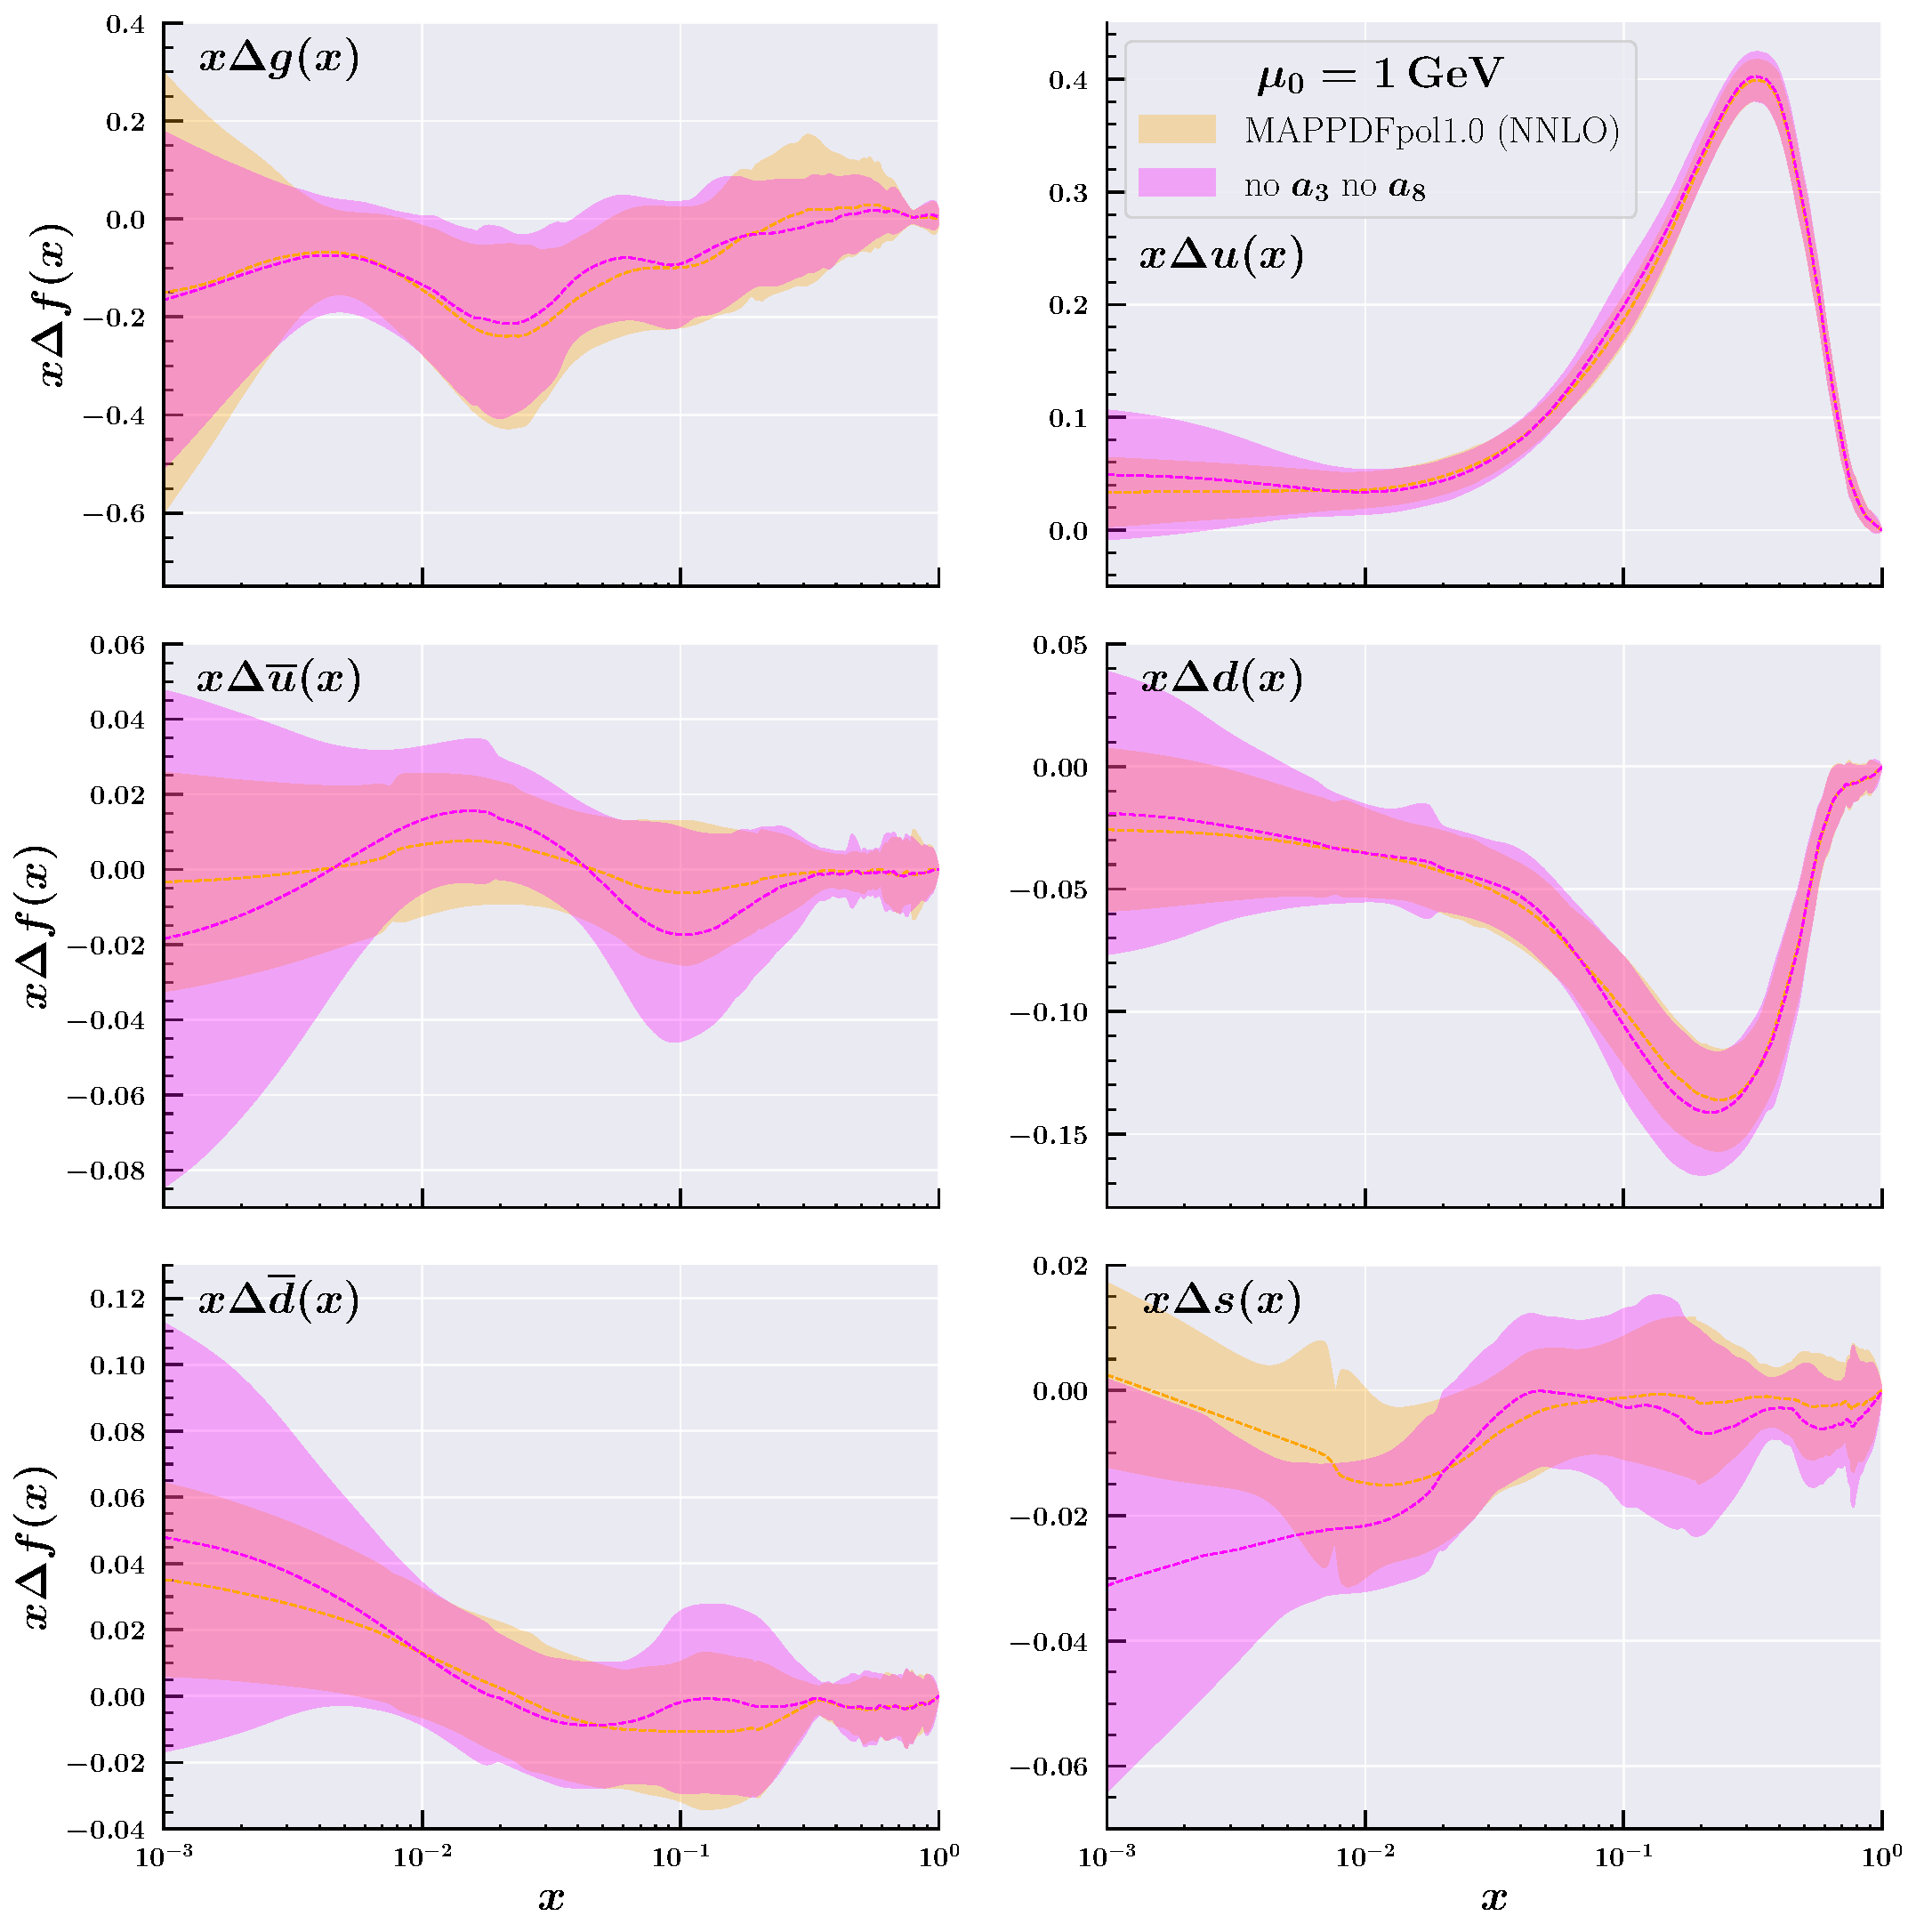
\includegraphics[width=\textwidth]{Chapters/Chapter_4/figs/a3_a8_nnlo.pdf}
  \caption{\small{Comparison of the \texttt{MAPpol1.0} baseline set at NNLO with and without including sum rules $a_3$ and $a_8$ in the data set. Parton distributions are displayed in flavour basis at $\mu_0 = 1 \, \T{GeV}$ as functions of $x$.}}
  \label{fig:a3_a8_nnlo}
\end{figure}

The baseline fit \texttt{MAPpol1.0} includes the sum rules $a_3$ and $a_8$ as part of the data set. In order to assess the impact of these two additional points, I performed two more PDF determinations at NLO and NNLO using the same baseline configuration Tab.~\ref{tab:baseline}, but without sum rules constraint. For each perturbative order, the comparisons are displayed in Figs.\ref{fig:a3_a8_nnlo} and \ref{fig:a3_a8_nlo}. The corresponding values of the global $\chi^2$ per data point for the constrained and unconstrained fits are presented in Tab.~\ref{tab:a3_a8_nnlo}, where the prediction of the moments of $\Delta T_3$ and $\Delta T_8$ distributions are also shown.%

\afterpage{
\begin{table}[t]
  \centering
  \small
  \begin{tabular}{c@{\hspace{1cm}}cc@{\hspace{1cm}}cc}
  \toprule \midrule
  \addlinespace
                                            & \multicolumn{2}{c}{\texttt{\textbf{MAPpol1.0}} (\textbf{NLO})} & \multicolumn{2}{c}{\texttt{\textbf{MAPpol1.0}} (\textbf{NLNO})} \\
  \cmidrule(lr){2-3} \cmidrule(lr){4-5}
                                            &   w/ $a_3$ and $a_8$    &    w/o $a_3$ and $a_8$                &   w/ $a_3$ and $a_8$    &    w/o $a_3$ and $a_8$    \tabularnewline
  \midrule
  \addlinespace
      $\chi^2/N_{\T{dat}}$                  &  $0.64$                 &  $0.64$                               &  $0.75$                 &  $0.73$           \tabularnewline
  \midrule
  \addlinespace
      $a_3 \, (x_{\T{min}} = 10^{-5})$      &  $1.269 \pm 0.005$      &  $ 1.171 \pm 0.417$                   &  $1.268 \pm 0.006$      &  $1.012 \pm 0.593$  \tabularnewline
  \midrule
  \addlinespace
      $a_8 \, (x_{\T{min}} = 10^{-5})$      &  $0.586 \pm 0.033$      &  $ 1.333 \pm 1.608$                   &  $0.588 \pm 0.032$      &  $2.243 \pm 2.252$  \tabularnewline
  \midrule \bottomrule
\end{tabular}
  \caption{
    \small
    Global $\chi^2$ and predictions of $a_3$ and $a_8$ for the two configurations w/ and w/o the sum rules constraint. The values are presented for both NLO and NNLO determinations.
  \label{tab:a3_a8_nnlo}}
\end{table}
%%
\begin{figure}[b]
  \centering
  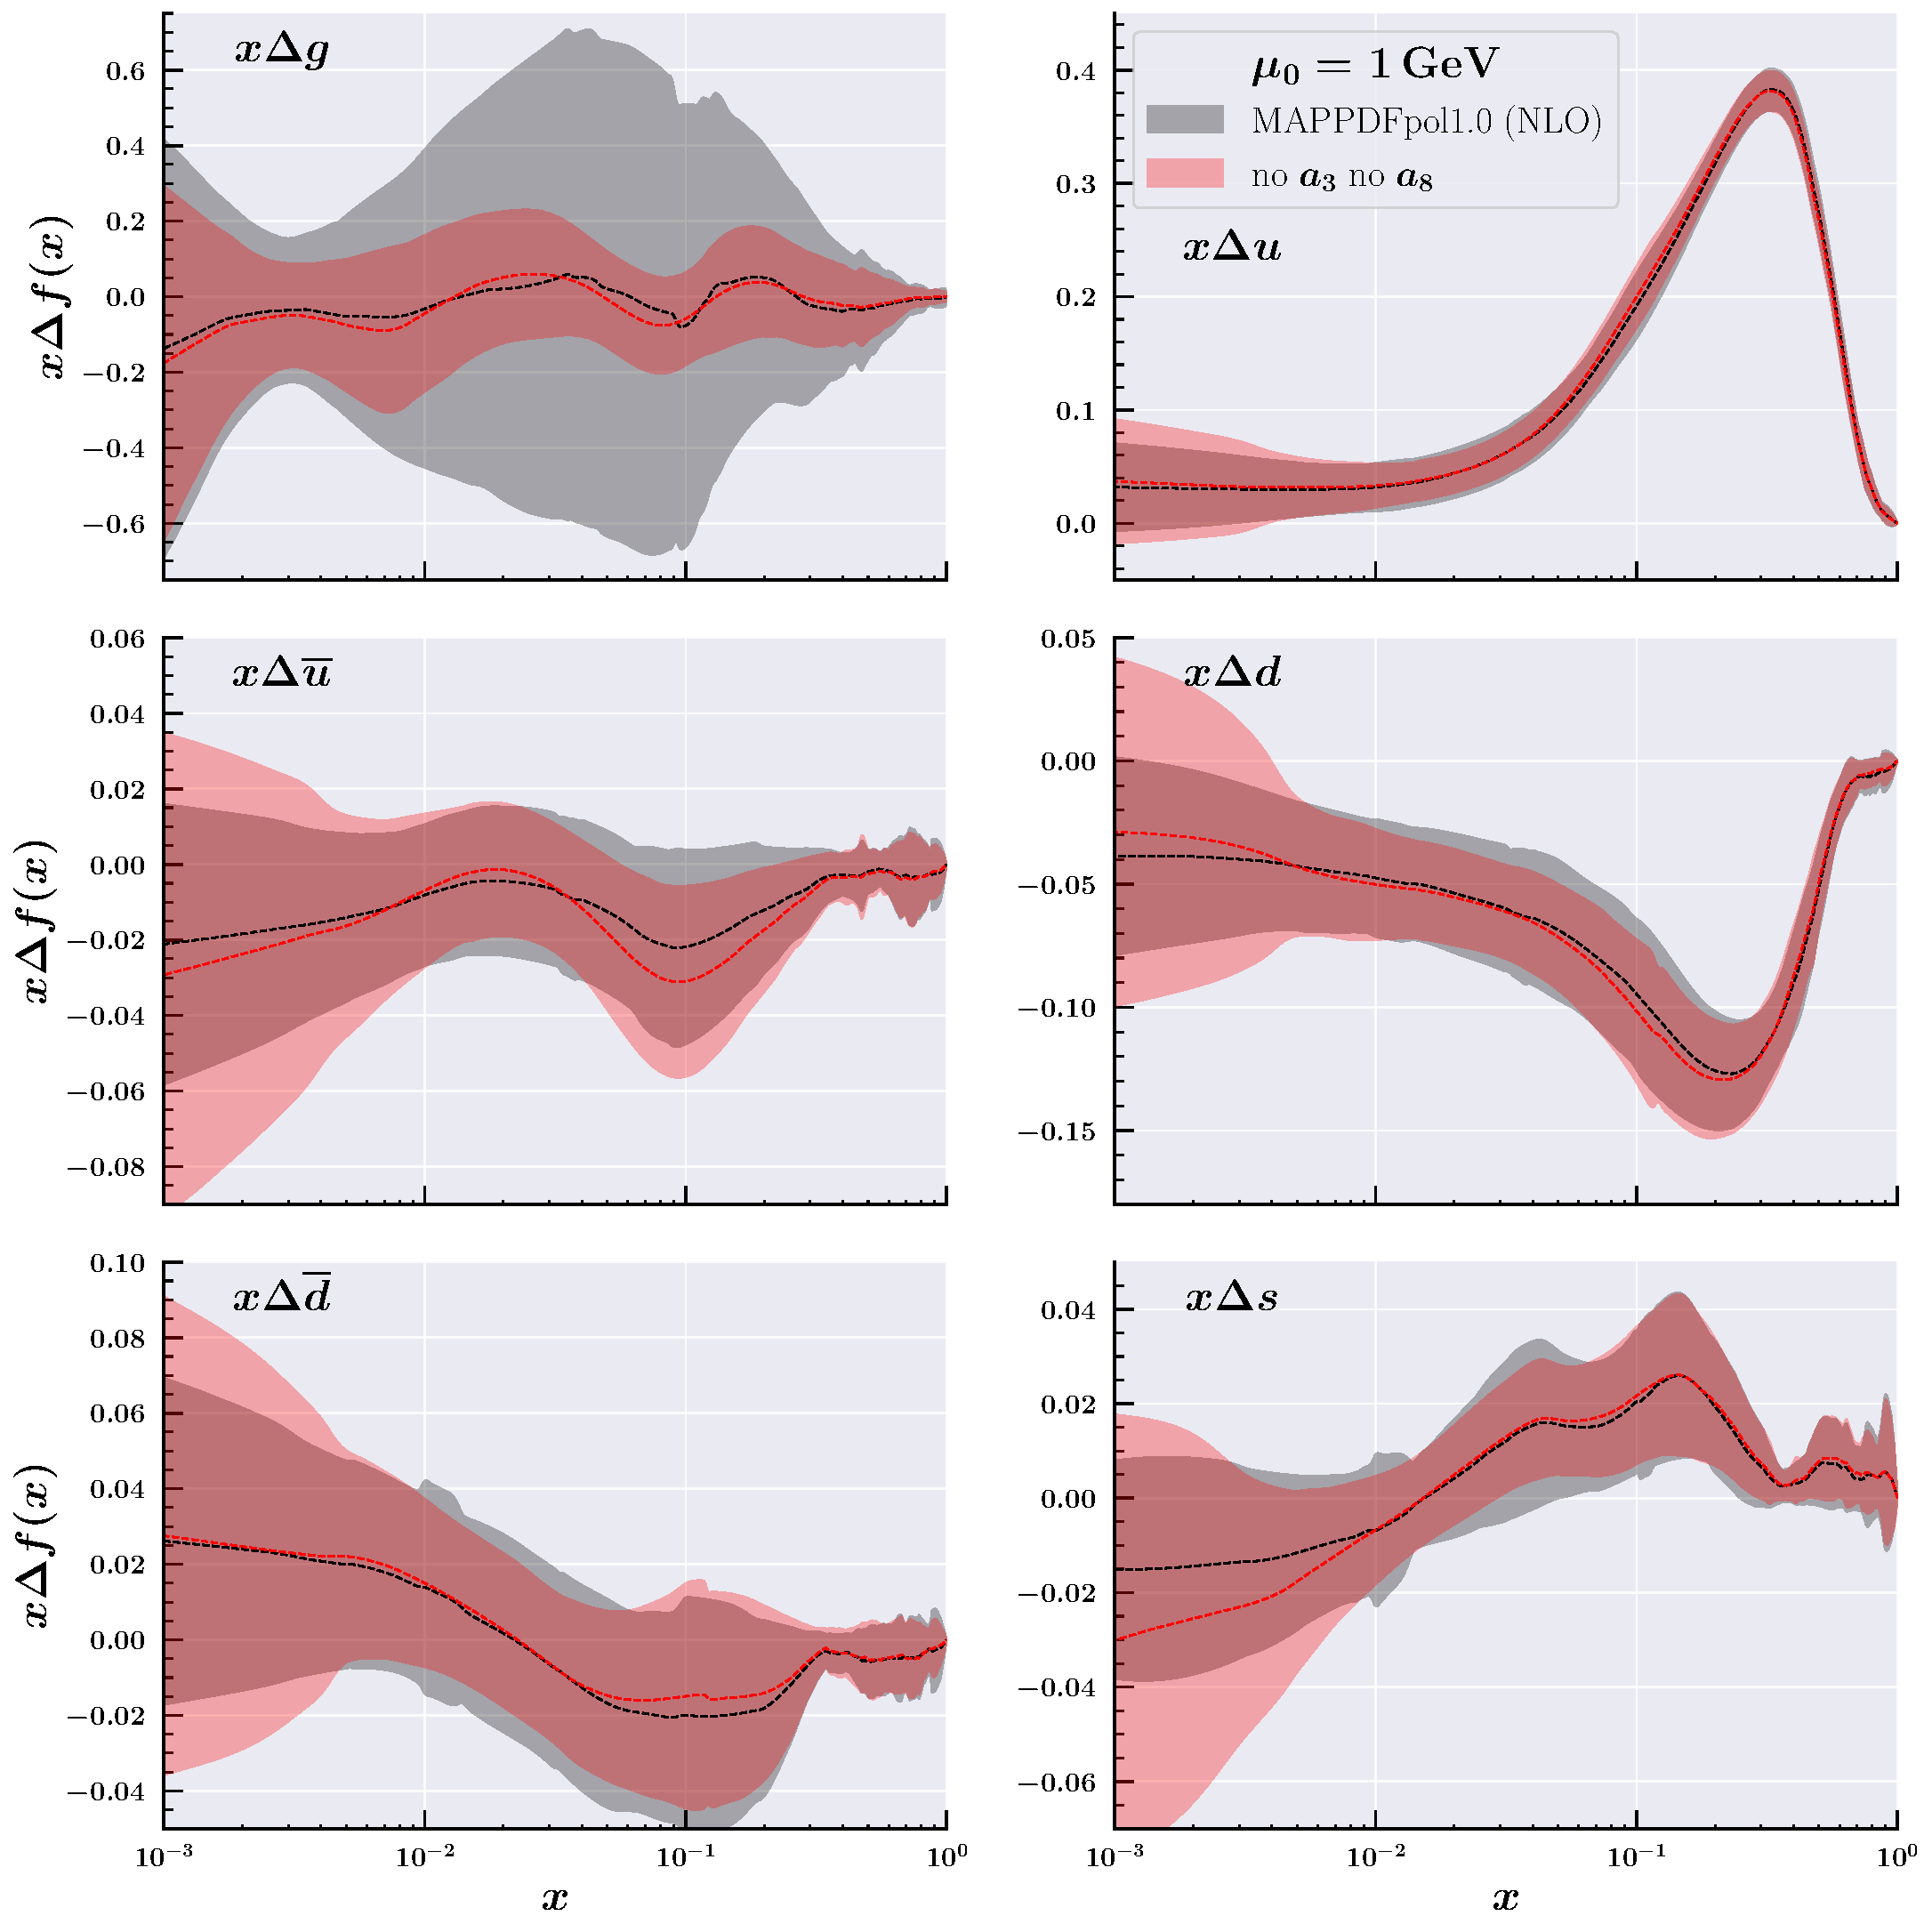
\includegraphics[width=\textwidth]{Chapters/Chapter_4/figs/a3_a8_nlo.pdf}
  \caption{\small{Same as Fig.~\ref{fig:a3_a8_nnlo}, but at NLO accuracy.}}
  \label{fig:a3_a8_nlo}
\end{figure}
\clearpage
}

At NNLO, a small deterioration of the fit quality is presented for the constrained determination. However, this may be due to the fact that sum rules reduce the space of all possible parton distributions, affecting the value of the global $\chi^2$. The inspection of Fig.~\ref{fig:a3_a8_nnlo} leads to the conclusion that, in general, the impact on helicity PDFs from constraining $a_3$ and $a_8$ is small, except for the sea quark distributions in the small-$x$ region. Moreover, the predictions reported in Tab.~\ref{tab:a3_a8_nnlo} for the NNLO case are in agreement within the uncertainties. Thus, at least at NNLO, the assumption of exact $SU(3)_f$ symmetry is compatible with the data included in the fit.%

For the NLO case, the picture is slightly modified. Fig.~\ref{fig:a3_a8_nlo} shows that the gluon is highly affected by the constraint, in particular in the medium-$x$ region. The other distributions are almost unchanged, although an inflation of the uncertainty bounds arises below $x \simeq 0.01$. The fit quality is unaffected by including the constraint, as shown in Tab.~\ref{tab:a3_a8_nnlo}. The values of $a_3$ and $a_8$ are recovered by the unconstrained distribution, although the moment of the octet is affected by a huge uncertainty.%

In conclusion, at NNLO the PDFs do not show much sensitivity to constraining $a_3$ and $a_8$, and the deterioration of the fit quality can be traced back to the reduction of the dimension of the functional space. At NLO the result is more stable in terms of fit quality, but the distribution of the gluon receives major changes. In both cases, the exact $SU(3)_f$ symmetry seems to be compatible with the included data.

%_______________________
\subsection*{Positivity}

The baseline configuration exploits positivity of the individual cross-sections entering the polarised asymmetries to impose the leading order constraint, Eq.~\eqref{eq:positivity_fl}, to each parametrised flavour separately, by using the \texttt{NNPDF31\_nnlo\_pch\_as\_0118} set ~\cite{NNPDF:2017mvq}. The constraint is implemented analytically as a transformation in the last layer of the neural network according to Eq.~\eqref{eq:pos_net}.%

In order to assess the effect of the positivity constraint, I performed another fit where the positivity has been imposed as in Eq.~\eqref{eq:positivity_fl_sigma}, but with an inflated value of the standard deviation. In particular, the constraint has been relaxed to $50 \, \sigma$. The parton distributions thus obtained are compared with the baseline fit and displayed in Fig.~\ref{fig:positivity} at NNLO. The values of the global $\chi^2$ are reported in Tab.~\ref{tab:positivity}.%

The fit quality receives no significant variations, with only a moderate improvement in the global $\chi^2$ when the constraint is relaxed. As in the case of the sum rules, this indicates that the parametrisation is flexible enough to enclose the positivity, and the deterioration of the fit quality is then ascribed to the reduction of the functional space caused by the constraint. In terms of PDFs, these are significantly affected by the positivity bound, in particular in the large-$x$ region, where the presence of data is scarce. Hence, the inclusion of the positivity constraint has a strong impact on the distributions, and guarantees that cross-sections are positive.
%However, it must be observed that the effects of the positivity bounds on parton distributions at small-$x$ region are not significant, given the LO and NLO positivity bounds differ significantly in this region \cite{Altarelli:1998gn}. Thus, the results of the baseline \texttt{MAPpol1.0} should be considered reliable out of the extrapolation region at small-$x$.

\afterpage{
\begin{table}[t]
  \centering
  \small
  \begin{tabular}{c@{\hspace{1cm}}c@{\hspace{1cm}}c}
  \toprule \midrule
  \addlinespace
                                        & \multicolumn{2}{c}{\texttt{\textbf{MAPpol1.0}} (\textbf{NNLO})} \\
  \cmidrule(lr){2-3}
                                        &   Positivity    &    Unp. PDF $+ \, 50 \, \sigma$ \tabularnewline
  \midrule
  \addlinespace
      $\chi^2/N_{\T{dat}}$               &  $0.86$                  &  $0.78$                \tabularnewline
  \midrule \bottomrule
\end{tabular}
  \caption{
    \small
    Values of the global $\chi^2$ per data point for the baseline fit and the configuration with the positivity constrained relaxed to $50 \, \sigma$, both at NNLO.
  \label{tab:positivity}}
\end{table}
%%
\begin{figure}[b]
  \centering
  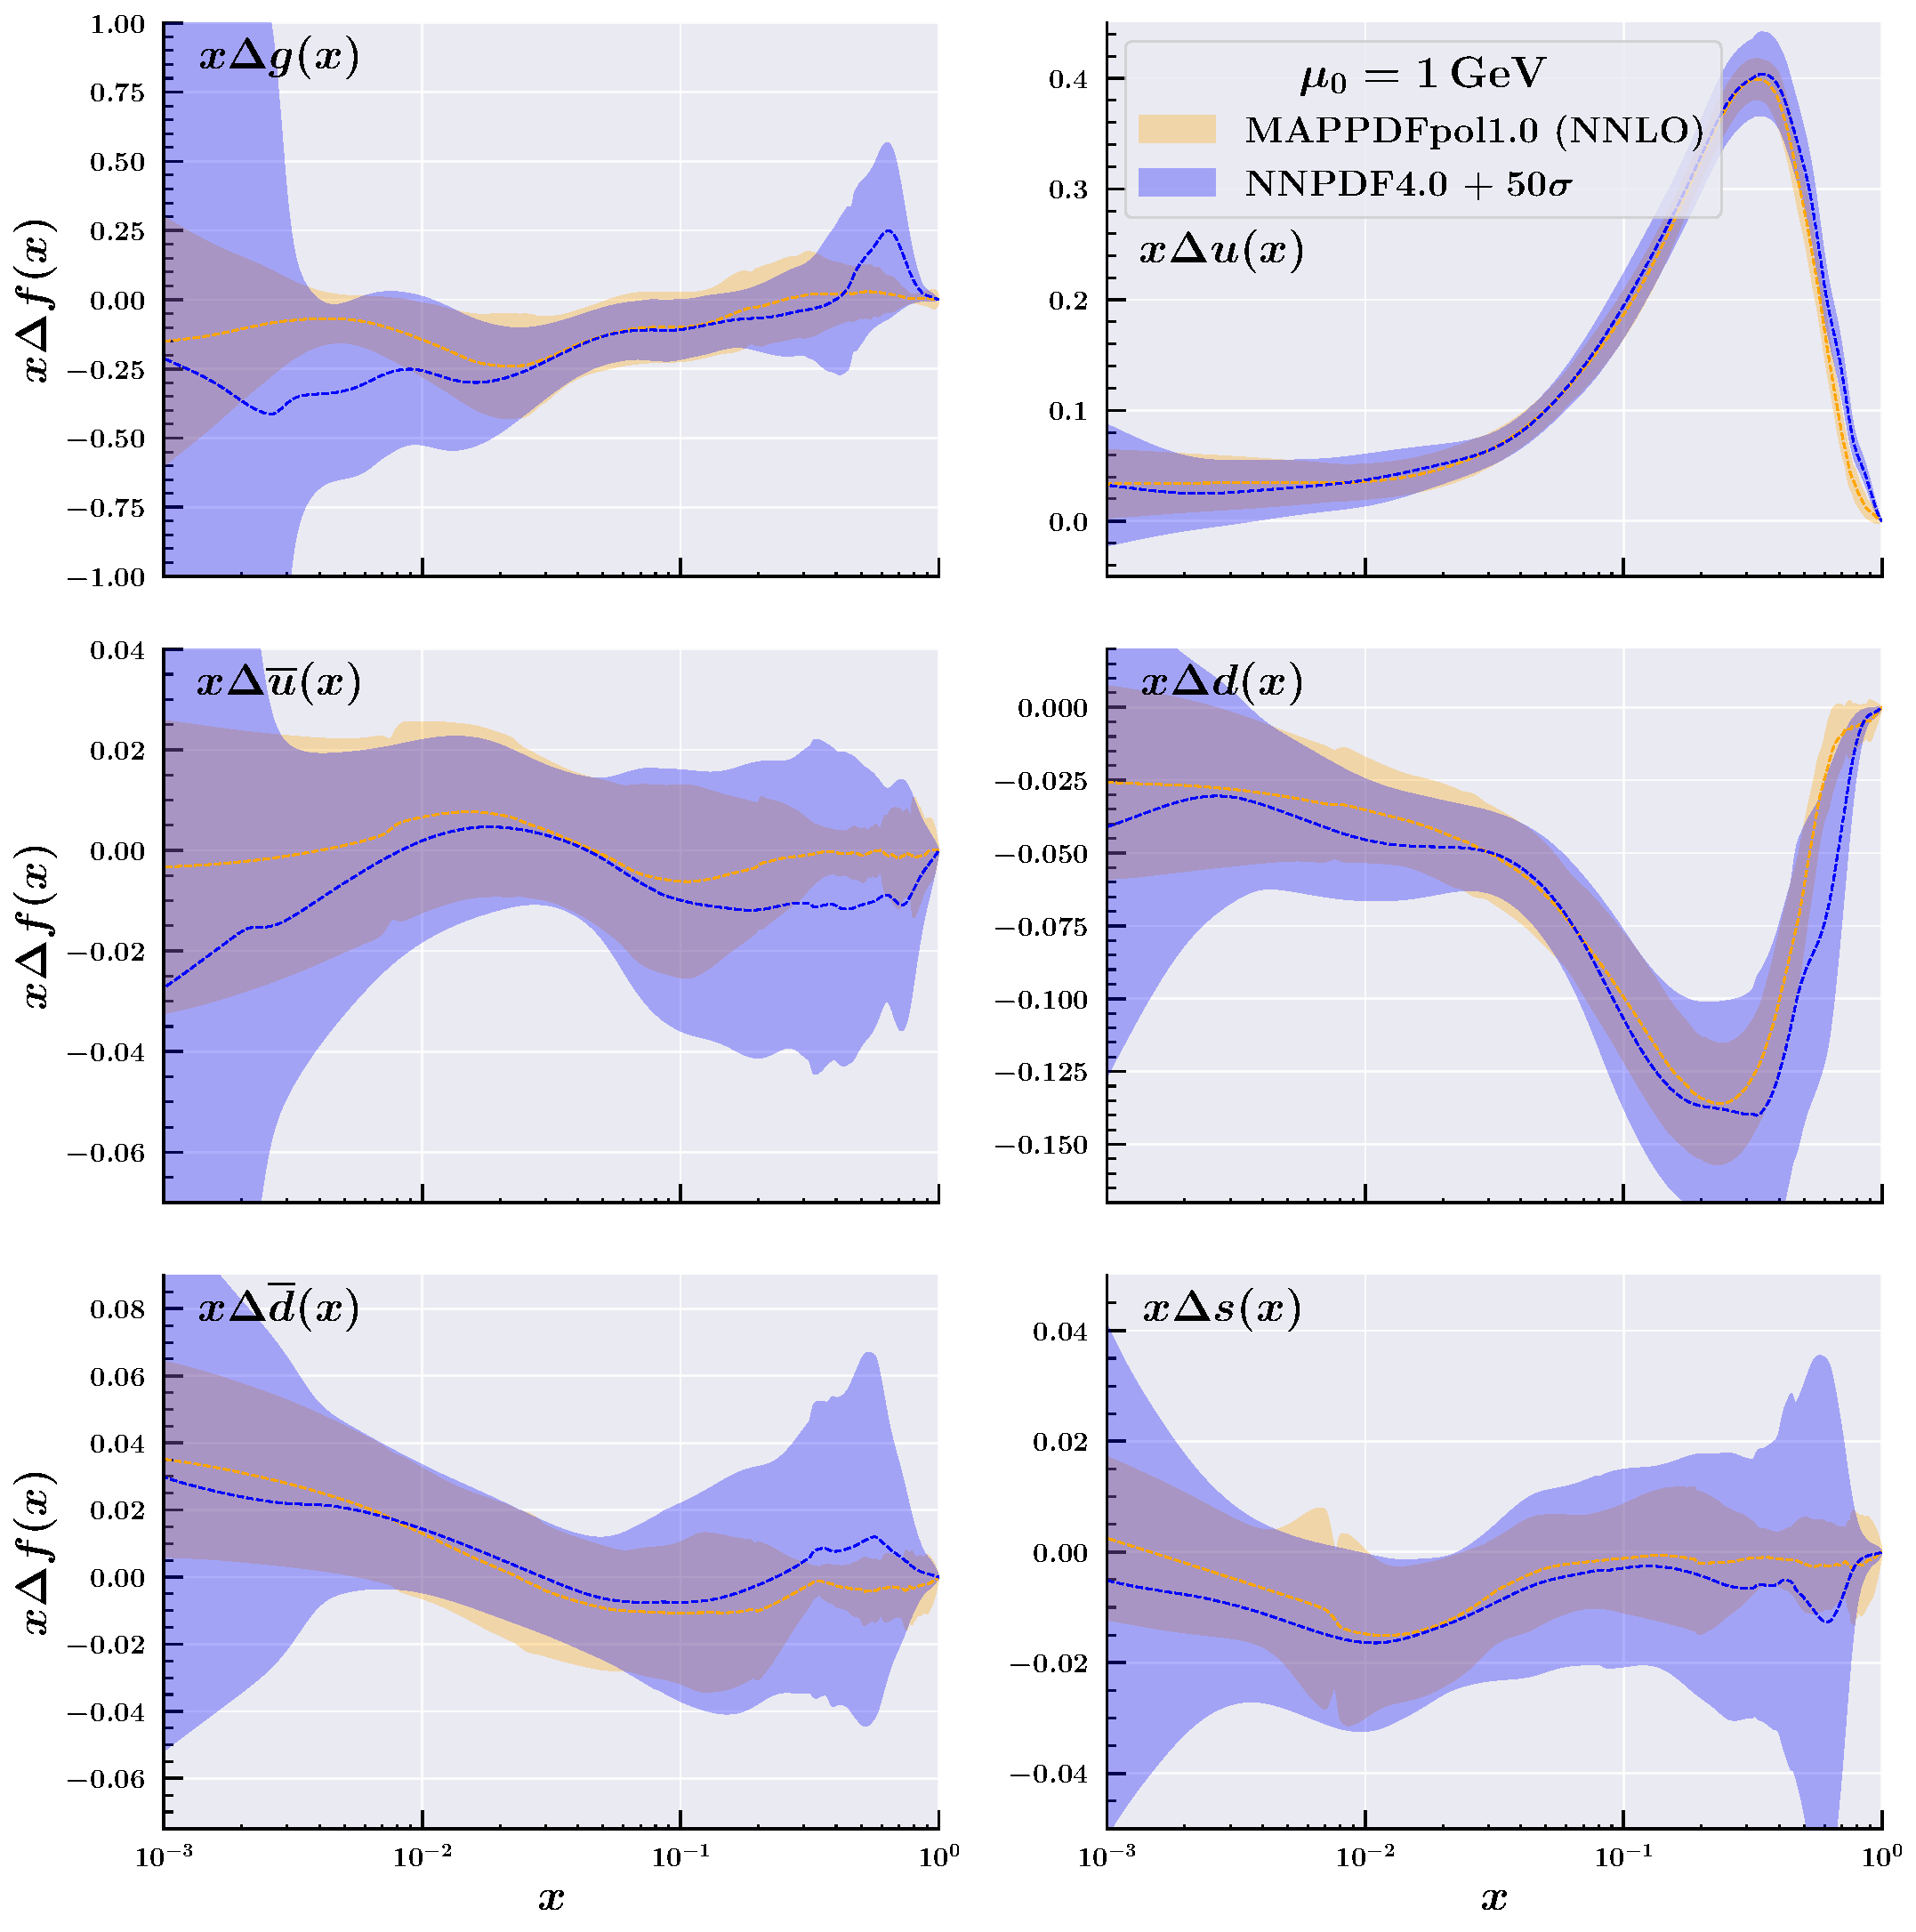
\includegraphics[width=\textwidth]{Chapters/Chapter_4/figs/positivity.pdf}
  \caption{\small{Comparison of the baseline \texttt{MAPpol1.0} fit at NNLO (orange) with the same set without imposing positivity (blue). Parton distributions are displayed in flavour basis at $\mu_0 = 1 \, \T{GeV}$ as functions of $x$.}}
  \label{fig:positivity}
\end{figure}
\clearpage
}

